\documentclass[a4, 12pt]{article}
\usepackage[paper=a4paper, top=2.5cm, left=2.5cm, right=2.5cm, bottom=2.5cm, headheight=1.0cm, headsep=1cm, footnotesep=0.5cm]{geometry}%
\clubpenalty = 10000
\widowpenalty = 10000
\usepackage[T1]{fontenc}
\usepackage{pslatex}%
\usepackage[utf8]{inputenc}
\usepackage{amsmath,amssymb}
\usepackage{bm}
\usepackage{tabularx}
\usepackage{graphicx}
\usepackage[english]{babel}
\usepackage{setspace}
\usepackage{setspace}
\usepackage{url}

% \usepackage{natbib}
\usepackage[style=apa,
			backend=biber,
			maxcitenames=1,
			maxcitenames=2,
			uniquelist=true]{biblatex}
\DeclareLanguageMapping{english}{english-apa}
\addbibresource{literature.bib}

\usepackage{float}
% \usepackage{placeins}
\usepackage{lscape}
\usepackage{rotating}
\usepackage{multirow}
\usepackage{longtable}
\usepackage{booktabs,caption}
\captionsetup[table]{skip=-2pt}
\usepackage{color}
\definecolor{red}{rgb}{1,0,0}

\usepackage{titlesec}
\usepackage{multicol}

\usepackage{array}
\usepackage{wrapfig}
\usepackage{colortbl}
\usepackage{pdflscape}
\usepackage{tabu}
\usepackage{threeparttable}
\usepackage{threeparttablex}
\usepackage[normalem]{ulem}
\usepackage{makecell}
\usepackage{xcolor}


\titleformat{\section}{\normalsize\bfseries}{\thesection}{1em}{}
\titleformat{\subsection}{\normalsize\bfseries}{\thesubsection}{1em}{}
\titleformat{\subsubsection}{\normalsize}{\thesubsubsection}{1em}{}

%CUSTOMISE LETTERING OF TITLE PAGE
% \makeatletter
% \renewcommand*{\@fnsymbol}[1]{\ensuremath{\ifcase#1\or *\or a  \else\@ctrerr\fi}}
% \makeatother

%TO ENABLE SUBSUBSECTION
\setcounter{secnumdepth}{3}
%TO SHOW SUBSUBSECTIONS IN TABLE OF CONTENTS
\setcounter{tocdepth}{3}

\usepackage{ifxetex,ifluatex}
\usepackage{fixltx2e} % provides \textsubscript
\ifnum 0\ifxetex 1\fi\ifluatex 1\fi=0 % if pdftex
  \usepackage[T1]{fontenc}
  \usepackage[utf8]{inputenc}
\else % if luatex or xelatex
  \ifxetex
    \usepackage{mathspec}
  \else
    \usepackage{fontspec}
  \fi
  \defaultfontfeatures{Ligatures=TeX,Scale=MatchLowercase}
\fi
% use upquote if available, for straight quotes in verbatim environments
\IfFileExists{upquote.sty}{\usepackage{upquote}}{}
% use microtype if available
\IfFileExists{microtype.sty}{%
\usepackage{microtype}
\UseMicrotypeSet[protrusion]{basicmath} % disable protrusion for tt fonts
}{}
\usepackage{hyperref}
\hypersetup{unicode=true,
            pdftitle={Untitled},
            pdfborder={0 0 0},
            breaklinks=true}
\urlstyle{same}  % don't use monospace font for urls
\usepackage{color}
\usepackage{fancyvrb}
\newcommand{\VerbBar}{|}
\newcommand{\VERB}{\Verb[commandchars=\\\{\}]}
\DefineVerbatimEnvironment{Highlighting}{Verbatim}{commandchars=\\\{\}}
% Add ',fontsize=\small' for more characters per line
\usepackage{framed}
\definecolor{shadecolor}{RGB}{248,248,248}
\newenvironment{Shaded}{\begin{snugshade}}{\end{snugshade}}
\newcommand{\KeywordTok}[1]{\textcolor[rgb]{0.13,0.29,0.53}{\textbf{#1}}}
\newcommand{\DataTypeTok}[1]{\textcolor[rgb]{0.13,0.29,0.53}{#1}}
\newcommand{\DecValTok}[1]{\textcolor[rgb]{0.00,0.00,0.81}{#1}}
\newcommand{\BaseNTok}[1]{\textcolor[rgb]{0.00,0.00,0.81}{#1}}
\newcommand{\FloatTok}[1]{\textcolor[rgb]{0.00,0.00,0.81}{#1}}
\newcommand{\ConstantTok}[1]{\textcolor[rgb]{0.00,0.00,0.00}{#1}}
\newcommand{\CharTok}[1]{\textcolor[rgb]{0.31,0.60,0.02}{#1}}
\newcommand{\SpecialCharTok}[1]{\textcolor[rgb]{0.00,0.00,0.00}{#1}}
\newcommand{\StringTok}[1]{\textcolor[rgb]{0.31,0.60,0.02}{#1}}
\newcommand{\VerbatimStringTok}[1]{\textcolor[rgb]{0.31,0.60,0.02}{#1}}
\newcommand{\SpecialStringTok}[1]{\textcolor[rgb]{0.31,0.60,0.02}{#1}}
\newcommand{\ImportTok}[1]{#1}
\newcommand{\CommentTok}[1]{\textcolor[rgb]{0.56,0.35,0.01}{\textit{#1}}}
\newcommand{\DocumentationTok}[1]{\textcolor[rgb]{0.56,0.35,0.01}{\textbf{\textit{#1}}}}
\newcommand{\AnnotationTok}[1]{\textcolor[rgb]{0.56,0.35,0.01}{\textbf{\textit{#1}}}}
\newcommand{\CommentVarTok}[1]{\textcolor[rgb]{0.56,0.35,0.01}{\textbf{\textit{#1}}}}
\newcommand{\OtherTok}[1]{\textcolor[rgb]{0.56,0.35,0.01}{#1}}
\newcommand{\FunctionTok}[1]{\textcolor[rgb]{0.00,0.00,0.00}{#1}}
\newcommand{\VariableTok}[1]{\textcolor[rgb]{0.00,0.00,0.00}{#1}}
\newcommand{\ControlFlowTok}[1]{\textcolor[rgb]{0.13,0.29,0.53}{\textbf{#1}}}
\newcommand{\OperatorTok}[1]{\textcolor[rgb]{0.81,0.36,0.00}{\textbf{#1}}}
\newcommand{\BuiltInTok}[1]{#1}
\newcommand{\ExtensionTok}[1]{#1}
\newcommand{\PreprocessorTok}[1]{\textcolor[rgb]{0.56,0.35,0.01}{\textit{#1}}}
\newcommand{\AttributeTok}[1]{\textcolor[rgb]{0.77,0.63,0.00}{#1}}
\newcommand{\RegionMarkerTok}[1]{#1}
\newcommand{\InformationTok}[1]{\textcolor[rgb]{0.56,0.35,0.01}{\textbf{\textit{#1}}}}
\newcommand{\WarningTok}[1]{\textcolor[rgb]{0.56,0.35,0.01}{\textbf{\textit{#1}}}}
\newcommand{\AlertTok}[1]{\textcolor[rgb]{0.94,0.16,0.16}{#1}}
\newcommand{\ErrorTok}[1]{\textcolor[rgb]{0.64,0.00,0.00}{\textbf{#1}}}
\newcommand{\NormalTok}[1]{#1}
\usepackage{graphicx,grffile}
\makeatletter
\def\maxwidth{\ifdim\Gin@nat@width>\linewidth\linewidth\else\Gin@nat@width\fi}
\def\maxheight{\ifdim\Gin@nat@height>\textheight\textheight\else\Gin@nat@height\fi}
\makeatother
% Scale images if necessary, so that they will not overflow the page
% margins by default, and it is still possible to overwrite the defaults
% using explicit options in \includegraphics[width, height, ...]{}
\setkeys{Gin}{width=\maxwidth,height=\maxheight,keepaspectratio}
\IfFileExists{parskip.sty}{%
\usepackage{parskip}
}{% else
\setlength{\parindent}{0pt}
\setlength{\parskip}{6pt plus 2pt minus 1pt}
}
\setlength{\emergencystretch}{3em}  % prevent overfull lines
\providecommand{\tightlist}{%
  \setlength{\itemsep}{0pt}\setlength{\parskip}{0pt}}
% Redefines (sub)paragraphs to behave more like sections
\ifx\paragraph\undefined\else
\let\oldparagraph\paragraph
\renewcommand{\paragraph}[1]{\oldparagraph{#1}\mbox{}}
\fi
\ifx\subparagraph\undefined\else
\let\oldsubparagraph\subparagraph
\renewcommand{\subparagraph}[1]{\oldsubparagraph{#1}\mbox{}}
\fi

%%% Use protect on footnotes to avoid problems with footnotes in titles
\let\rmarkdownfootnote\footnote%
\def\footnote{\protect\rmarkdownfootnote}

\begin{document}
\begin{titlepage}
% Titlepage (fold)
\thispagestyle{empty}%
\begin{center}
\renewcommand{\baselinestretch}{1.0}\normalsize %
\textbf{
The effect of music education on students' well-being. Empirical evidence from a field experiment}\\[1cm]
Preliminary - work in progress \\[1cm]
This draft: \today \\[1cm]
% Comments welcome \\[0.25cm]
% \renewcommand{\baselinestretch}{1.5}\normalsize
Vera Schramm \\
University of Halle-Wittenberg \\[0.75cm]
% \today
 \end{center}


\end{titlepage}

\pagenumbering{roman}
\setcounter{page}{2}
\AtBeginEnvironment{tabular}{\singlespacing}
\AtBeginEnvironment{lltable}{\singlespacing}
\captionsetup[table]{font={stretch=1.5}}

\renewcommand{\baselinestretch}{1}\normalsize

\textbf{\normalsize Abstract}
\emph{Objective.} This thesis examines the effect of a music project which was carried out parallel at different middle schools in Bavaria on life satisfaction and on certain areas of satisfaction. \emph{Methods.} I review prior work pertaining to music's impact mainly on cognitive outcomes. My analysis applies Bayesian inference and multilevel modeling on a longitudinal data set to asses music involvement and possible effects on life satisfaction, satisfaction with friends, satisfaction with the class and satisfaction with the school. A difference-in-difference framework allows to draw causal conclusion even despite the fact that the treatment group and the control group differ in some aspects \emph{Results.} The students from the treatment group tend to have a more \_\_\_\_\_\_\_\_\_\_ Although \_\_\_\_\_\_\_\_\_, this effect is only minimal\ldots{} \emph{Conclusion.} Music participation in form of the studied music project cuased little changes\ldots{}

\clearpage
\tableofcontents

\clearpage
\listoftables

\clearpage
\listoffigures

\clearpage
\doublespacing
\pagestyle{plain}
\pagenumbering{arabic}

\hypertarget{introduction}{%
\section{Introduction}\label{introduction}}

\label{introduction}

In German schools, subjects like arts and music are often considered less important than the typical hard subjects like math and science. Due to a lack of teachers, many classes are canceled, of which 80\% are in the subject of music. In Saxony we see ongoing efforts to eliminate the subject of music from the curriculum entirely. Furthermore, the quality of music lessons suffers from the fact that 80\% of its teaching staff are foreign to the subject (Möller, 2017).

Music education experts are concerned about this development. According to them, music should not be regarded as a private matter. Regardless of their socioeconomic background, school children must have the opportunity to receive high level music education because it is as important for a proper education as literacy and mathematics (Gebert, 2018). Prof.~Höppner, the General Secretary of the German Music Council (Generalsekretär des Deutschen Musikrats), said in an interview that music education helps to build stable self-esteem by learning to access ones own emotions (Stoverock, n.d.). He points out that the phase where music can shape a young person explicitly well is completed by the age of 13. That stresses the importance of high quality music education for students in pre- and secondary school.

The Federal Association of Music Education (Bundesverband Musikunterricht (BMU)) has set up the ``Agenda 2030'' to initiate an improvement in music education. Similar to Höppner (Stoverock, n.d.), they consider music education valuable and essential for a social and cultural society. It encourages children to take responsibility and to increase their sense of self-determination (Bundesverband Musikunterricht (BMU), 2016, p. 2).

In views of this broad societal debate, empirical research has concentrated on the effect of music education on cognitive abilities (school grades and IQ in particular). Not so much effort was spent on observing the connection of music and well-being. This seems surprising because life satisfaction and happiness have become central research areas in the social sciences. My thesis addresses this research gap and investigates the effects of music education on children's overall life satisfaction and on satisfaction in specific areas, namely satisfaction with the class, satisfaction with friends, and satisfaction with the school. It analyzes music education in the classroom where fifth and sixth grade students have one additional hour of music education per week. The project that is studies is called ``klasse.im.puls'' and it promotes the establishment of musical training in secondary schools in Bavaria. The program was implemented with the intention to give every child the opportunity to learn how to play an instrument. Additional positive outcomes were expected: an increase in self-confidence and social competence, as well as a reduction in violent behavior.\footnote{For more information:} The project was supervised by the FAU Erlangen-Nuremberg Music Teaching Department in collaboration with the Bavarian Ministry of Education.
My analysis focuses on the change in the overall life satisfaction as a consequence of participating in the music project. Further outcome variables are of interest: Satisfaction with friends, satisfaction with the class, and satisfaction with the school. I will approach the problem using a multilevel model that accounts for differences among students and differences among schools by introducing a hierarchical structure where students represent level 1 and schools level 2. Data are available for different points in time. Therefore a third level, time periods are included. To estimate the treatment effects, Bayesian analysis is the method of choice. Using Bayesian inference allows to make predictions on the outcomes of future projects of this kind. As the KIP project is still continuing to be applied in many schools over Bavaria, the predicted effects also carry important information.

I am particularly interested in life satisfaction as an outcome of the music project because there is the idea of higher values of LS coming with many benefits also in later life. Among other positive correlates, adolescents reporting very high levels of LS are less likely to be affected by depression, anxiety, negative affect and social stress compared to adolescents with very low life satisfaction. Also, they achieve higher SEAs and demonstrate higher mean scores of school satisfaction (Gilman \& Huebner, 2006, p. 316; Proctor, Linley, \& Maltby, 2009, p. 928). These results go in line with a study by Suldo \& Huebner (2004, p. 94) that shows that LS could be a moderating variable in predictions of the development of psycho-pathological behaviors. Low life satisfaction may be an indication for externalizing behavior problems in the future. When life satisfaction is on a higher level, those behavior problems are less likely to occur (Suldo \& Huebner, 2004, p. 100) The authors conclude that life satisfaction might operate as a buffer against the development of subsequent externalizing behavior problems ``in the face of stressful life events'' (Suldo \& Huebner, 2004. p.~101). Kim, Conger, Elder, \& Lorenz (2003) add to the discussion that externalizing behavior problems in turn lead to more stressful life events. That reciprocal interrelation of stressful life events and externalizing problems (reported as delinquent behaviors) leads to unhealthy dynamics of increasing stress and behavior problems. If higher LS leads to better coping mechanisms with stressful life events, these dependencies could be reduced.
LS is also positively correlated with children having higher measures of self-esteem, internal locus of control, and extraversion (Huebner, 1991a, p. 107). These features help in building a solid foundation for later life. On the other hand, dissatisfaction with life is associated with adolescents having poor mental health (like anxiety and neuroticism) and physical health and being exposed to a higher risk of considering or attempting suicide (Huebner, 1991a, p. 107; Valois, Zullig, Huebner, \& Drane, 2004, p. 94). Furthermore, Zullig, Valois, Huebner, Oeltmann, \& Drane (2001, pp. 284--185) show that adolescents reporting low levels of overall life satisfaction are more likely to use drugs and alcohol earlier in life and in higher amounts than adolescents with medium or high life satisfaction.

Considering the statement of Höppner, one would expect the project to positively effect students' life satisfaction. Evidence for this relation would lend credibility to the project and support its continuation. It could also stress the importance of music education and signal the Ministry of Culture to keep music education in the curriculum and work on its implementation in federal states alongside Bavaria. My thesis is a first try to reveal some information about the influence of the KIP project on the students. However, regardless of the findings, there will be no discussion on the reasons of any observed effects from a music education background. The analysis will be strictly observable and any interpretation of the results must be left to music and education experts.

The structure of my thesis is as follows: At first there will be an overview of the current literature on music effecting students' lives in chapter \ref{ch:roleofmusic}. Next, in chapter \ref{ch:data} the project and the data set will be explained along with descriptive statistics and a detailed diagnostic on pre-treatment differences in the treatment group compared to the control group. The data section also critically discusses challenges arising with measuring self reported life satisfaction in children. The identification strategy is presented in chapter \ref{sec:identification}, following the estimation in the \ref{ch:estimation}th chapter. Finally, chapter \ref{ch:results} shows the results and chapter \ref{ch:conclusion} concludes and discusses.

\clearpage

\hypertarget{the-role-of-music-in-childrens-lives}{%
\section{The role of music in childrens' lives}\label{the-role-of-music-in-childrens-lives}}

\label{ch:roleofmusic}
With regard to the effect of music on students' lives, most of the researchers are interested in academic outcomes and intelligence among students who are actively involved in music. Generally, there is the predominant perception of a positive link between music and cognitive abilities. Osborne, McPherson, Faulkner, Davidson, \& Barrett (2015, p. 14) observed improved math skills and higher subjective well-being scores in children that were part of a music project. He also found them to have a better self-control over impulsive behavior. Yang (2015) (p.~385),Wetter, Koerner, \& Schwaninger (2008) (p.~372) , Hille (2014) (p.~62), and Guhn, Emerson, \& Gouzouasis (2019) (p.~316) present evidence that children playing music have better grades at school. But this conclusion is not very meaningful as all of these studies follow a correlational design and do not allow for causal inference. Nonetheless, the very optimistic and as we will see not quite realistic belief has prevailed that playing music causes children to achieve better results at school. This conclusion needs to be revised. In an extensive review of the available evidence concerning associations between music and cognitive abilities, the picture is not so clear any longer (Schellenberg \& Weiss, 2013). Small associations between music training and mathematical ability in correlational and quasi-experimental studies might result from individual differences in general intellectual ability (p.~527). The available evidence simply indicates that high-functioning children (i.e., higher IQ, better performance in school) are more likely than other children to take music lessons and to perform well in mathematics and other tests of cognitive ability (p.~534). This fits with the Hille (2014) study where the outcome difference in cognitive skills between musically active and inactive children reduces greatly when holding constant observable characteristics. An other plausible interpretation of study outcomes that fail to detect a causal relationship comes from Wetter et al. (2008). He points out the possibility that the relationship is explained by affluent parents being more likely to afford music lessons for their child and thus, the socio-economic background may be the cause of higher performance at school. Despite the weakness of the above studies to draw causal inference, there is slight evidence that there may be a causal direction \emph{from} music training \emph{to} cognitive abilities in a study by Schellenberg (2004). He compares two treatment groups who receive piano lesson and voice lesson respectively to a control group in which the children have drama lessons. Random assignment to the different conditions allowed for inference that music lessons caused small increases in cognitive abilities (namely larger increases in full-scale IQ). However, this does not preclude the possibility that high-functioning children are more likely driven to play music. The misconception of music being a predictor for academic achievement is also discussed by Southgate \& Roscigno (2009) (p.~17) who states that music is rather a mediator, to some degree, of family background and student status. Results from a meta-analysis, suggest that music training does not reliably enhance children and young adolescents' cognitive or academic skills, and that previous positive findings were probably due to confounding variables, such as placebo effects and lack of random allocation of participants (Sala \& Gobet, 2016, p. 64). The effect size was reduced in studies that applied a proper study design (random allocation of participants to the treatment group and comparison to an active control group). With respect to the mathematical outcomes, the only study comparing a music training to an active control group and with random allocation of the participants to the group (Mehr, Schachner, Katz, \& Spelke, 2013) found a negative effect size. These considerations are in clear contrast to the popular perception that music training enhances any non-music related cognitive skill.

However positive outcomes due to music could be found outside academics. The Norwegian psychologist and musicologist Even Ruud who in 1978 was the head of the first music therapy training performed extensive studies on music and identity. He states that cultural activities, explicitly music, can ``contribute to a feeling of quality of life and the subjective sense of health.'' (p.~96). In an experimental study by Costa-Giomi (2004) a positive causal effect was detected of piano lessons on self-esteem {[}144{]} but she did not find an effect on math computation scores. One especially popular project that was conducted to improve children's lives is Venezuela's National Music Education Program ``El Sistema''. It is a large scale social music education program established by José Abreu in the 1970s. 300,000 children are equipped with instruments every year and receive regular after-school lessons and are playing in orchestras. The initial goal was to prevent children from using drugs and being involved in violence and crime which was successfully achieved. Being in orchestras also enhanced social behavior of the students through greater concern for others and their own well-being (Uy, 2012, p. 13). However positive effects go far beyond keeping adolescents away from drugs and violence: El sistema teaches the participating students to ``reflect and act upon the world in order to transform it'' {[}7{]}. Playing in an orchestra means joy, motivation, teamwork, the aspiration to success {[}6{]}. The students pick up management and organizational skills and responsibility due to many roles and rules that they need to follow to sty in the program{[}p.~10{]}. Also, being in an orchestra gives the students the change to conceptualize themselves as part of something much larger and greater (p.~11) and they learn to express greater concern for others' and their well being (p.~13). However, it remains open if those positive effects are a result of being musically active or if they are induced by the natrue of an orchestra being a place of social interaction that positively affects childrens' lives. Anyway, El Sistema became internationally popular and was replicated in several countries. Osborne et al. (2015) reviewed the outcome of El Sistema inspired projects in Australia and found significantly higher subjective well-being scores in the participating group (p.~14). Students from the music program also had better self-control over impulsive behavior (p.~15). However, other studies come to contrary conclusions and fail to show a significant effect of music participation on well-being, social skills, emotional intelligence or self-esteem (Portowitz, Lichtenstein, Egorova, \& Brand, 2009, p. 121; Schellenberg, 2011, p. 190 association). Again, findings are diffuse and therefore interpretation of any results needs to be done with caution.

The takeaway from this section is that causal conclusion must be done carefully and with adequate methods. This thesis is an attempt to do this and to complements existing literature by using different music indicators and by adjusting estimation strategies to provide further insight on the relationship between music and education. A multilevel model will help to draw correct inference by avoiding an overstatement of statistical significance. This often happens when failing to recognize hierarchical structures because then standard errors of regression coefficients will be underestimated. It also allows for inference beyond the groups that are observed because in a multilevel model, the groups in the sample are treated as a random sample from a population of groups. \url{http://www.bristol.ac.uk/cmm/learning/multilevel-models/what-why.html}

\clearpage

\hypertarget{data}{%
\section{Data}\label{data}}

\label{ch:data}
In this section, I will first give more background information on the project itself, including the data collection process, before describing the data and variables individually. After general summary statistics, there is a section about handling potential issues arising with differences in the treatment and control group.

\hypertarget{the-project}{%
\subsection{The project}\label{the-project}}

\label{sec:project}
The data come from the years 2012-2014 when KIP was conducted in six different secondary schools (Mittel- und Realschulen) in Nuremberg. Generally, there are different types of implementations of the KIP project (e.g.~choir, brass band, string orchestra) among which the rock band model was implemented in all of the schools that are subject to this study. Probably due to parents' and students' music preferences, this type has been the most popular. In that concept, a class was typically divided into four bands, practicing concurrently in two rooms with one teacher each, talking turns by one band playing their instrument and another doing the vocals.

A school had to fulfill certain criteria in order to get support in the form of advanced training for music teachers and acquiring equipment in order to implement ensemble music class teaching. For example, the school had to make sure that there was a full-time music teacher who was qualified to carry out the project. That person was trained to lead a band class and attended yearly meetings with other music teachers to share experiences. This way, it can be assured that the treatment in each school looked pretty much the same and there were no noteworthy differences in the way the teachers arranged the music lessons in the band classes. Participating schools were supported in acquiring equipment and instruments to implement ensemble music class teaching. In each school was a band class and a control class. The band classes received three music lessons per week, whereas the control classes only received two lessons of regular music education. Music education in the treatment classes differed significantly from that in the control group. In the band classes, the teachers had a more practical approach and there was less theoretical music education than in the control group. The three music lessons per week were split into a) Instrumental instructions in small groups, b) ensemble playing, and c) general music education (music theory or history). The latter was similar to how regular music education was implemented in the control group. Therefor not only the amount of music education is higher in the treatment group but also the way that music education is delivered differs a lot from normal music lessons. It is more practical and the equipment is of higher quality. The students played concerts in regular intervals and were thus able to share what they had learned.

In five different points of time, the students received the same anonymized questionnaire which they were asked to complete within about 30 minutes.

The assessments were performend in:
wave 1 -- Beginning of 5th grade (pre-treatment) \textbackslash{}
wave 2 -- Mid of 5th grade \textbackslash{}
wave 3 -- end of 5th grade \textbackslash{}
wave 4 -- mid of 6th grade \textbackslash{}
wave 6 -- end of 6th grade \textbackslash{}

\hypertarget{variables}{%
\subsection{Variables}\label{variables}}

\label{sec:variables}
The sample that is studied has a hierarchical structure with three levels: Each student is observed multiple times, ideally at five points throughout the project if he was present on every assessment day. The different time periods are level one. The students themselves are level two and as the students are nested within schools, the third level is the school level. More details on the specific variables follow now:

\hypertarget{satisfaction}{%
\subsubsection{Satisfaction}\label{satisfaction}}

The term \emph{life satisfaction} refers to a cognitive evaluation of a person's reaction to his or her life in contrast to \emph{affect}, an ongoing emotional reaction. Combined, LS and affect yield subjective well-being (Diener, 2009, p. 71).

To measure life satisfaction and any area of satisfaction, I use an 11-point scale, with responds on a scale from 0 to 10 with ``0'' being completely unsatisfied and ``10'' being completely satisfied. Life satisfaction is the variable of interest in my thesis, alongside with Satisfaction with friends, Satisfaction with class, and Satisfaction with school. An extract of the questionnaire with the exact wording of the question can be found in the index (Figure \ref(fig:questionnaire). Measuring life satisfaction on a 0-10-scale is quite common in that field of literature {[}Mellor, Stokes, Firth, Hayashi, \& Cummins (2008) Cheung \& Lucas (2014)\} but also 7-point scales are found a lot (Diener, Emmons, Larsen, \& Griffin, 1985). For the model, the satisfaction measures are assumed to be cardinal comparable both across and within individuals across time. There is broad consensus in the literature to interpret satisfaction responds as cardinally scaled (Ferrer-i-Carbonell \& Frijters, 2004). Mean values and standard deviations of life satisfaction and the different areas of satisfaction from wave 1 are presented in Table \ref{tab:mean-LS}.

\begin{table}[H]

\caption{\label{tab:mean-LS}Mean satisfaction}
\centering
\begin{tabular}[t]{lrr}
\toprule
Variable & Mean & SD\\
\midrule
Life satisfaction & 7.29 & 2.56\\
Satisfaction friends & 8.86 & 1.82\\
Satisfaction class & 7.58 & 2.05\\
Satisfaction school & 7.74 & 2.20\\
\bottomrule
\end{tabular}
\end{table}

As the standard deviations are quite big, the life satisfaction reports are presented in Figure \ref{fig:hist-lsat} for a better overview. As already cited above in Chambers \& Johnston (2002), children tend to report values at the extreme ends of a scale. This is also what happened in the KIP sample: The histogram hows a striking portion of the students indicating to have a life satisfaction of 10. Also, a high amount of the students respond with a 5 on the scale. Almost 50\% of the students assign themselves a life satisfaction of 5 or of 10. This might indicate the issue that children at that age are having a hard time understanding what the question asked them to do. It also suggests difficulties to make the transfer from their individual assessment of their life satisfaction to pair it with a number and so they just chose 5 randomly, hoping that it was neither ``right or wrong''.

\begin{figure}[H]

{\centering 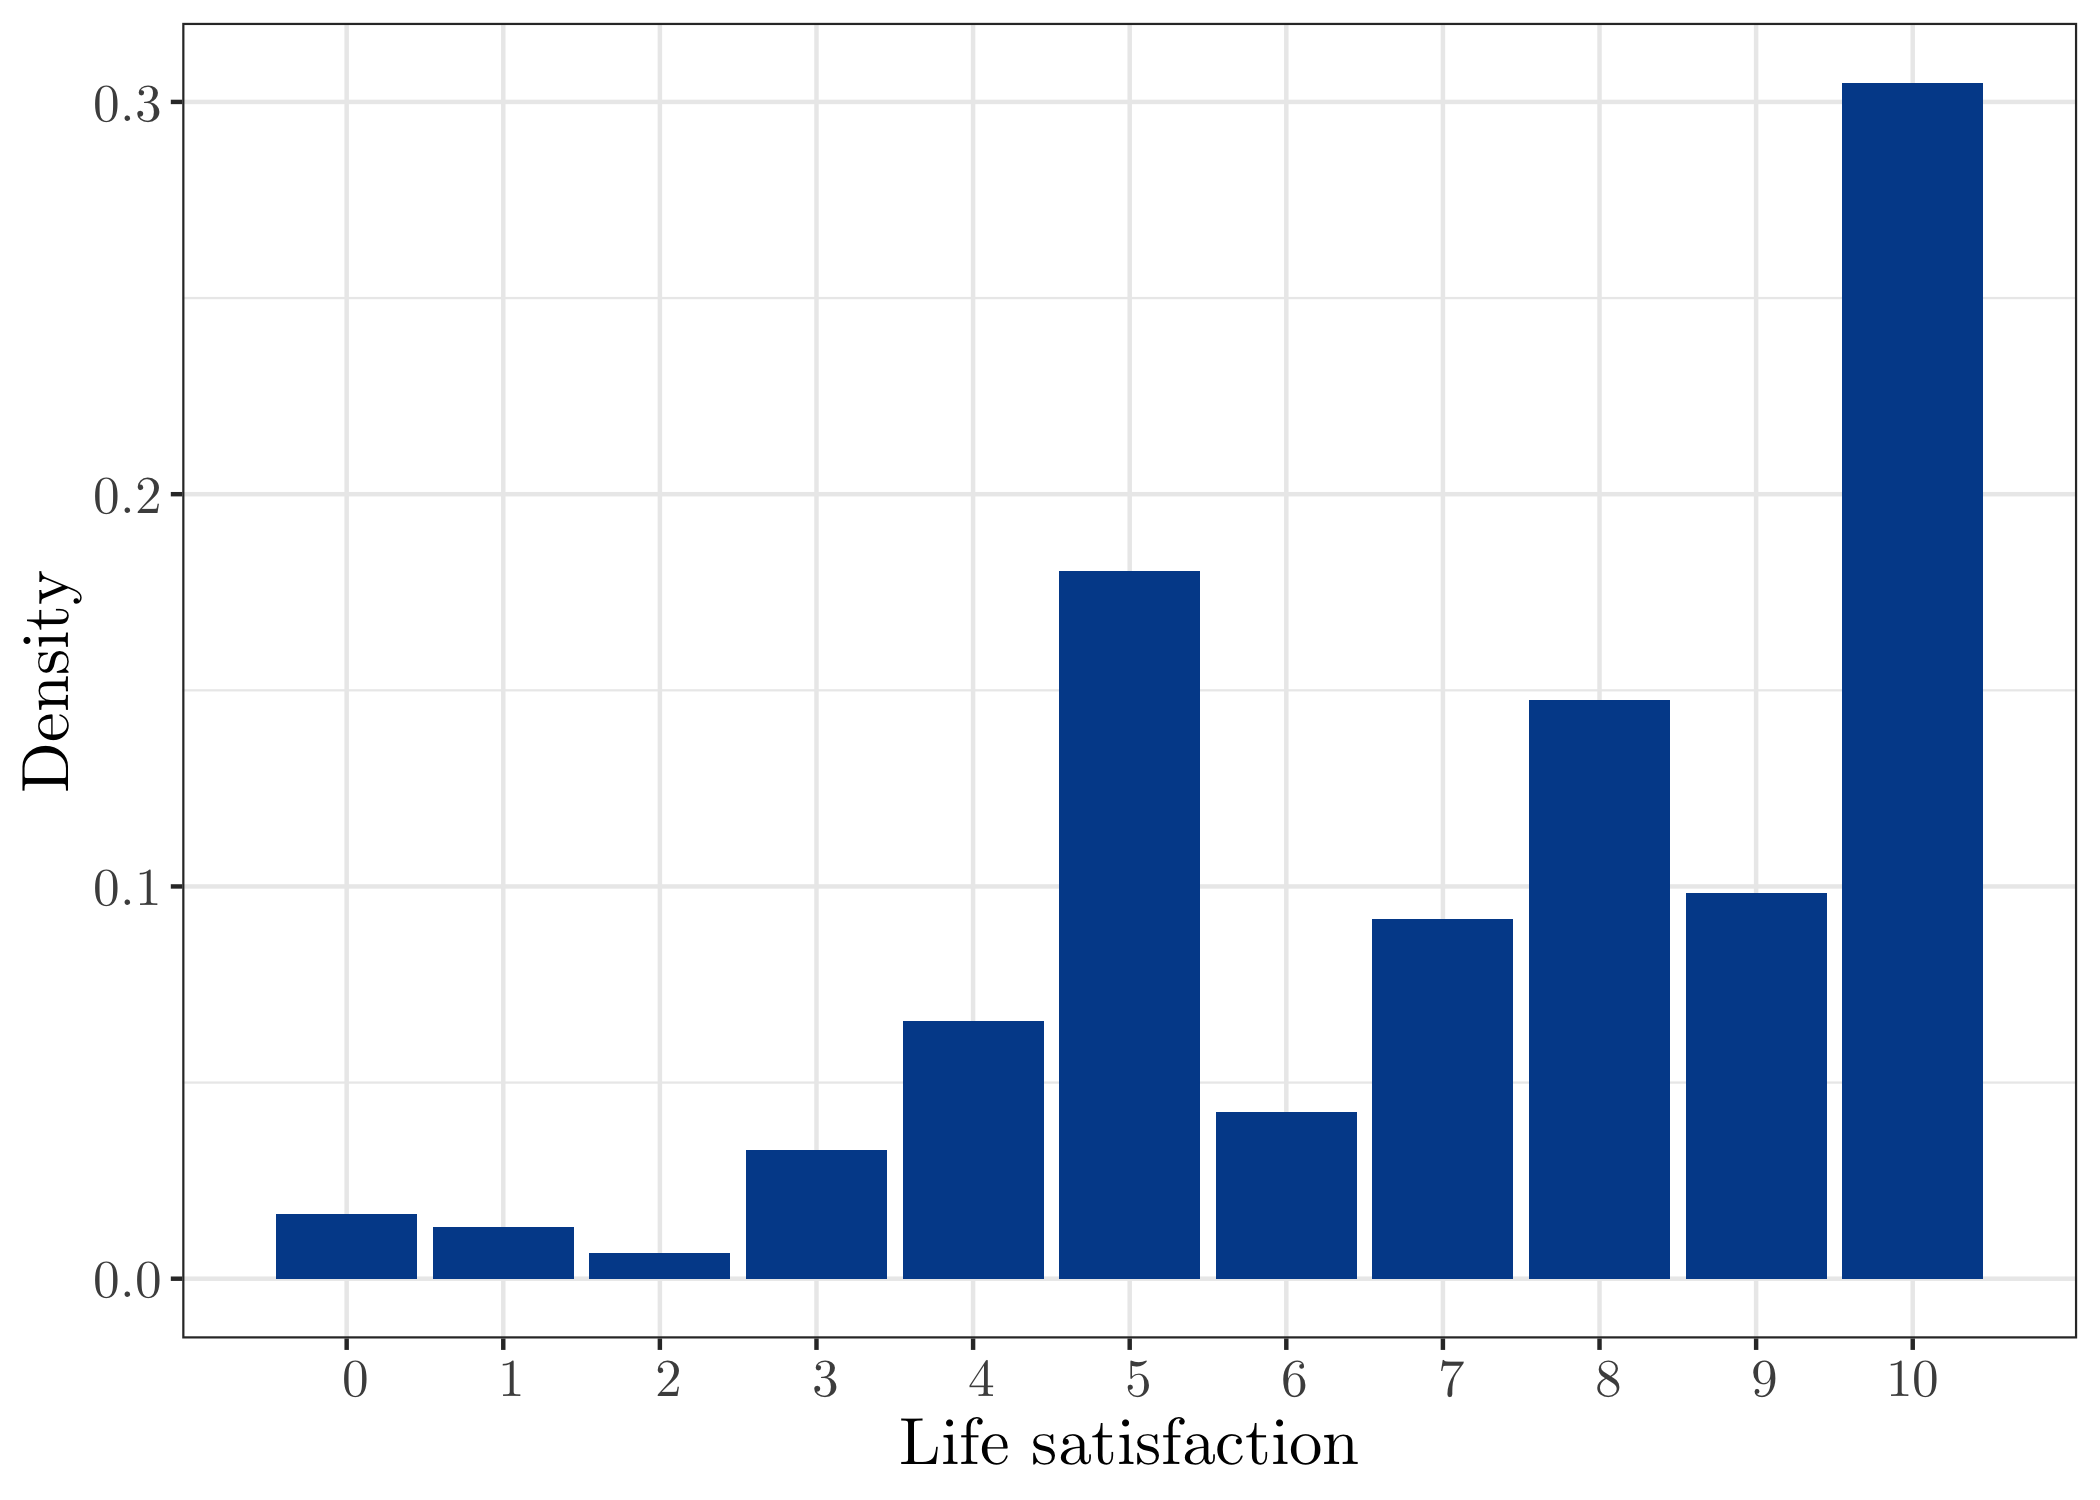
\includegraphics[width=0.8\linewidth,]{../figures/lsat_bar} 

}

\caption{Distribution of life satisfaction in wave 1}\label{fig:hist-lsat}
\end{figure}

\hypertarget{treatment}{%
\subsubsection{Treatment}\label{treatment}}

The treatment is represented by a binary variable, indicating whether a student participated in the treatment (``1'') or not (``0''). The treatment is conducted on the class level. All students in the same class are assigned the same indicator of whether or not they attend the treatment. Students did not change the class. Treatment also appears in the data set as an interaction term with each time period in that a treatment effect can be measured. Multiplying the binary indicator of treatment with the dummy variable for each period gives four indicators with the variable indicating 1 if the observation was in the treatment group and was made in the respective wave and 0 otherwise.

\hypertarget{individual-characterisitc-background}{%
\subsubsection{Individual characterisitc background}\label{individual-characterisitc-background}}

In the first wave, students were asked to state their gender (Tick either \emph{``Are you a girl/are you a boy?''}). This question did not appear in subsequent waves which leads to the issue that children who were not in school on the day the first questionnaire was handed to them, appear as NAs in the sample. The same happened for migration background. To avoid drop out of too many observations in the estimation process, gender and migration background were manipulated as category variables and NAs were replaced by the category \emph{unknown}. This leads to the following distribution of time-invariant individual characteristics: Both the gender and the migration background is not known for around 20\% of the total of 390 students. The available data show that out of the remaining students, 45\% are female and 36\% have a migration background.

The fact that it is an unbalanced panel where not all the children attended each wave should be considered more thoroughly. In Table \ref{tab:N-Obs-per-wave-school} , the number of students in each school and each wave is presented. It shows that the number of students is varying from one wave to another, most severely in class five. In that class, the number of participants of the questionnaire drops by a third in wave 5 compared to the first period. The overall effect of this decline on the whole sample is shown in table \ref{tab:N-Obs}. In the treatment group, the number of students decreases from 154 in wave 1 and is the lowest in wave 4 with 137 participants. In the control group, there are 144 to start with and only 134 in wave 5. This could be a reason to exclude school five from the observation completely as the attrition rate in the remaining schools is not that alarming. In total there were 1500 students observed throughout the five waves, however I excluded the students that did not report their satisfaction. If I had left them in the sample, this would have lead to problems in the posterior predictive checks because when the `brmsfit' fits the model, any N/As are excluded automatically. Without these observations, there are 1429 left.

\begin{table}[H]

\caption{\label{tab:N-Obs-per-wave-school}Number of observations by school}
\centering
\begin{tabular}[t]{lrrrrrr}
\toprule
School & Wave 1 & Wave 2 & Wave 3 & Wave 4 & Wave 5 & Sum\\
\midrule
1 & 47 & 40 & 46 & 48 & 52 & 233\\
2 & 53 & 49 & 52 & 48 & 49 & 251\\
3 & 49 & 46 & 48 & 52 & 52 & 247\\
4 & 47 & 45 & 47 & 50 & 49 & 238\\
5 & 56 & 57 & 57 & 43 & 37 & 250\\
6 & 46 & 42 & 44 & 38 & 40 & 210\\
Sum & 298 & 279 & 294 & 279 & 279 & 1429\\
\bottomrule
\end{tabular}
\end{table}

As a third individual background variable, I included if a student had some musical experience before the project had started. I expected students who already played an instrument before or received private music lessons would be more drawn to the treatment class. Also, as I want to find out if the project made students more satisfied, any previous effects of music on satisfaction should be minimized.

\begin{table}[H]

\caption{\label{tab:N-Obs}Number of observations by treatment}
\centering
\begin{tabular}[t]{lrrrrr}
\toprule
  & Wave 1 & Wave 2 & Wave 3 & Wave 4 & Wave 5\\
\midrule
Treatment group & 154 & 142 & 146 & 137 & 145\\
Control group & 144 & 137 & 148 & 142 & 134\\
\bottomrule
\end{tabular}
\end{table}

\hypertarget{pre-treatment-differences}{%
\subsection{Pre-treatment differences}\label{pre-treatment-differences}}

\label{sec:pre-treat-diff}
The treatment groups were not randomized, but formed by choice. This makes it a quasi-experimental study where the decision who attended the treatment group was made before the entrance to grade 5. Parents could choose to put their child into a music class. Therefore, the experiment is not fully randomized. Children who were already practicing music in the first place might have been more likely to enter the music class. Also, the decision can be a a consequence of parental and socio-economic background of the student. To have a better idea of possible differences between the treatment and the control group, I computed standardized mean differences:

\begin{table}[H]

\caption{\label{tab:std-mean-diff}Standardized mean differences}
\centering
\begin{tabular}[t]{lr}
\toprule
  & treated = 1 vs 0\\
\midrule
lsat & 0.15\\
female & 0.15\\
sat\_friends & 0.15\\
sat\_class & 0.15\\
class.prob & 0.07\\
\addlinespace
class.excl & 0.09\\
note.deu & 0.10\\
note.mat & 0.13\\
note.mus & 0.17\\
\cellcolor[HTML]{b3cde0}{hob.mus.making} & \cellcolor[HTML]{b3cde0}{0.51}\\
\addlinespace
dauer.mus.lis & 0.12\\
\cellcolor[HTML]{b3cde0}{dauer.mus.making} & \cellcolor[HTML]{b3cde0}{0.42}\\
play.instr & 0.05\\
mus.active & 0.12\\
migback & 0.14\\
\bottomrule
\end{tabular}
\end{table}

The standardized mean differences are not a reason for concern in this setting. For most of the observed variables, there are no notable differences between the treatment group and the control group. However, as already suspected, there are differences in prior musical knowledge. Among the treated, there are relatively more children who have music as a hobby before the project has even started. Of the 87 students who answered with ``yes'' to the question if music was their hobby, only 24 were assigned to the control group and the remaining 63 students attended the band classes. Also, the duration of making music is very different in the two subgroups. In the Treatment group, 56\% are practicing at least 30 min, while in the control group that share is only 35\%. However, the model addresses this issue by applying a difference-in-difference approach to estimate the causal effect of additional music lessons on students' well-being. Possible differences in the control group and the treatment group are not a problem for inference.

\hypertarget{measuring-ls-in-children}{%
\subsection{Measuring LS in children}\label{measuring-ls-in-children}}

\label{sec:measurement}
To investigate ones quality of life, research uses both objective and subjective indicators. Typical objective indicators are the income levels, crime rates, and access to medical services -- measures that are external and quantifiable. Subjective indicators on the other hand comprise subjective evaluations of ones' individual life circumstances (Gilman \& Huebner, 2000, p. 178). Only a modest relation between both measures was found which indicates that each approach carries unique information that are relevant for a comprehensive understanding of overall life quality (Veenhofen, 1996). Over time, measurement methods for subjective indicators have evolved, leading to substantial growth in the life satisfaction research. However, for a long time, most of the measurements were designed to assess adults' life satisfaction. Only recently, investigating correlates of life satisfaction in adolescents has begun. One reason why life satisfaction research in children was put off for a long time is probably that measuring life satisfaction in children is more challenging than for adults. Instruments for assessing children's subjective life satisfaction reports have been less intensively developed which is probably due to the fact that a Likert-type ratings scale is more difficult to use for younger children than for adolescents (Chambers \& Johnston, 2002, p. 28). For example, younger children or children with poorer readings skills are less able to respond appropriately to negative items on questionnaires and this effect biases the interpretation of children's responses (Marsh, 1986, p. 45). It is also common for children rating their subjective life satisfaction to show elevated extreme scores. As children become older, this tendency subsides and they are more capable of providing graded ratings in between the two extremes. These results have potentially substantial implications for the interpretation of self-report ratings form children \emph{this tendency might have an erroneous and invalid impact on the interpretation of children's self-reports}(Chambers \& Johnston, 2002, pp. 33--34). When dealing with self-reported life satisfaction in children, it is crucial that the respective child fully understands the question in order to give a valid response (Gluskie, 2012; Tomyn, Fuller-Tyszkiewicz, Cummins, \& Norrish, 2016). One must make sure that a child is old enough to know how to use a satisfaction scale. This requires children to distance themselves from the current situation, cognitively evaluate their life satisfaction (considering all relevant areas of life) and rate the degree to which certain items on the scale apply to them. This requires abstract thinking, which children develop in early adolescent years (10-14 years) (Gluskie, 2012; Piaget, 1955, 1969). Gilman \& Huebner (2000) have reviewed five different (both unidimensional and multidimensional) measurements explicitly developed to asses adolescents' life satisfaction.\footnote{The Students' Life Satisfaction Scale (Huebner, 1991b), the Satisfaction With Life Scale (Diener et al., 1985), the Perceived Life Satisfaction Scale (Adelman, Taylor, \& Nelson, 1989), the Comprehensive Quality of Life Scale - School Version (Cummins, 1997; Gullone \& Cummins, 1999), and the Multidimensional Student's Life Satisfaction Scale (Huebner, 1994)} The authors evaluated those measures in terms of validity and reliability and found all of the scales to be appropriate for research with adolescents {[}181-188{]}. The demographic characteristics of the available samples show that all of the adolescents observed were older than 12 years. Therefor it remains unclear if children younger than that age are able to report valid satisfaction.
An other instrument was developed by (Cummins \& Lau, 2005), the Personal Well-being Index (PWI-SC). Again, studies demonstrated reliability for this instrument as well (Casas \& Rees, 2015; Casas et al., 2011; Tomyn \& Cummins, 2011; Tomyn, Stokes, Cummins, \& Dias, 2019). But also in those studies, all of the adolescents were at least 12 years of age, mostly even older. There is only very little evidence on the psychometric properties of the PWI-SC for children below the age of 12.
One of them is González-Carrasco, Casas, Malo, Viñas, \& Dinisman (2016, p. 70) who applied the instrument for children as young as only 9 years and also found adequate fit of the data.
On the other hand, Tomyn et al. (2016) conducted a study with children aged 10-12 and concluded that subjective well-being data of children must be interpreted with caution. They also show that response bias towards the extreme positive end of a scale is higher with decreasing age. The authors do not recommend using the PWI-SC for children younger than 12 years. As for the specific sample, the PWI-SC did not serve as a valid instrument for measuring the SWB.

In conclusion, measuring life satisfaction in children is more challenging than for adults and is still in progress. It is advisable to check the validity and reliability of their data when testing children. Considering, the majority of the children from the KIP project are 10 year sold in wave 1 (72\% of those participating in wave 1), they might be just too young to give valid responses when asked about their life satisfaction. This must be kept in mind when evaluating the results.

\clearpage

\hypertarget{identification-strategy}{%
\section{Identification strategy}\label{identification-strategy}}

\label{sec:identification}
As I already mentioned in the introduction, I will make use of a multilevel model, precisely a varying-intercept and varying-slope multilevel model. A multilevel model is a good choice for drawing causal inference but also for prediction and descriptive modeling (Andrew Gelman, 2013, p. 6).
In the following, I will summarize important aspects of the methodology of those models and explain how multilevel models are best to navigate between underfitting (too few parameters included in the model) and overfitting (too many parameters included in the model). In the second part, I will give an introduction to Bayesian analysis that is ideal for multilevel modeling because of its underlying assumption that all parameters are random quantities.

\hypertarget{multilevel-modeling}{%
\subsection{Multilevel modeling}\label{multilevel-modeling}}

Since the sample is structured hierarchically, with students nested within schools, observed in several time periods, using a simple nonhierarchical model would be inappropriate. It would tend to underfit when there are only few parameters and to overfit the data when too many parameters are included. Though fitting the data well, often seems to be the goal of data analysis, these models are usually very poor in making predictions for new data (Andrew Gelman (2013), 101). (fit to sample always - not true of multilevel models - improves as we add parameters.

A multilevel model is a linear model in which parameters are given a probability model. Mcelreath (2020) (p.~14) suggests to think of parameters as a placeholder for a missing model. That probability model itself has parameters called hyperparameters which are also estimated from the data. In other words, they are parameters for parameters. Technically, there is no limit to the number of levels, however infeasible computation and ability to understand the model are in practice a restriction. Though multilevel models are more complicated, it is worth using them because they produce better estimates.

Multilevel models involve predictors at different levels of variation. In the KIP setting that means that it is possible to measure different effect sizes throughout time in each of the schools. It is likely to observe different response behaviors among the schools. Depending on the school, students might react differently to the project. This is an important investigation to find out if the intervention was more effective in some schools than in others. One school might have done something explicitly well or had to face challenges other schools did not. Learning from these findings could possibly help to improve the project in the future.

In a classical regression, assigning varying effects to each group is done by using interaction terms or running separate regressions for each subgroup of the sample. However, this has the disadvantage that estimates can be very imprecise, in particular when there are only few observations per group. Estimating parameters for each group separately is referred to as \emph{no-pooling} because each group is observed independently without considering the rest of the sample. On the other hand, ignoring the hierarchical structure and \emph{completely pooling} the information is also not recommended, because existing effects might disappear as illustrated in @(fig:lsat-vs-time). If solely taking the mean over all schools (solid purple line), there is almost no change in life satisfaction through time. But when each school taken separately, there are clear dynamics that substantially differ from each other. While in some schools, average life satisfaction is decreasing with different rates, in other school opposite trends are visible.

\begin{figure}[H]

{\centering 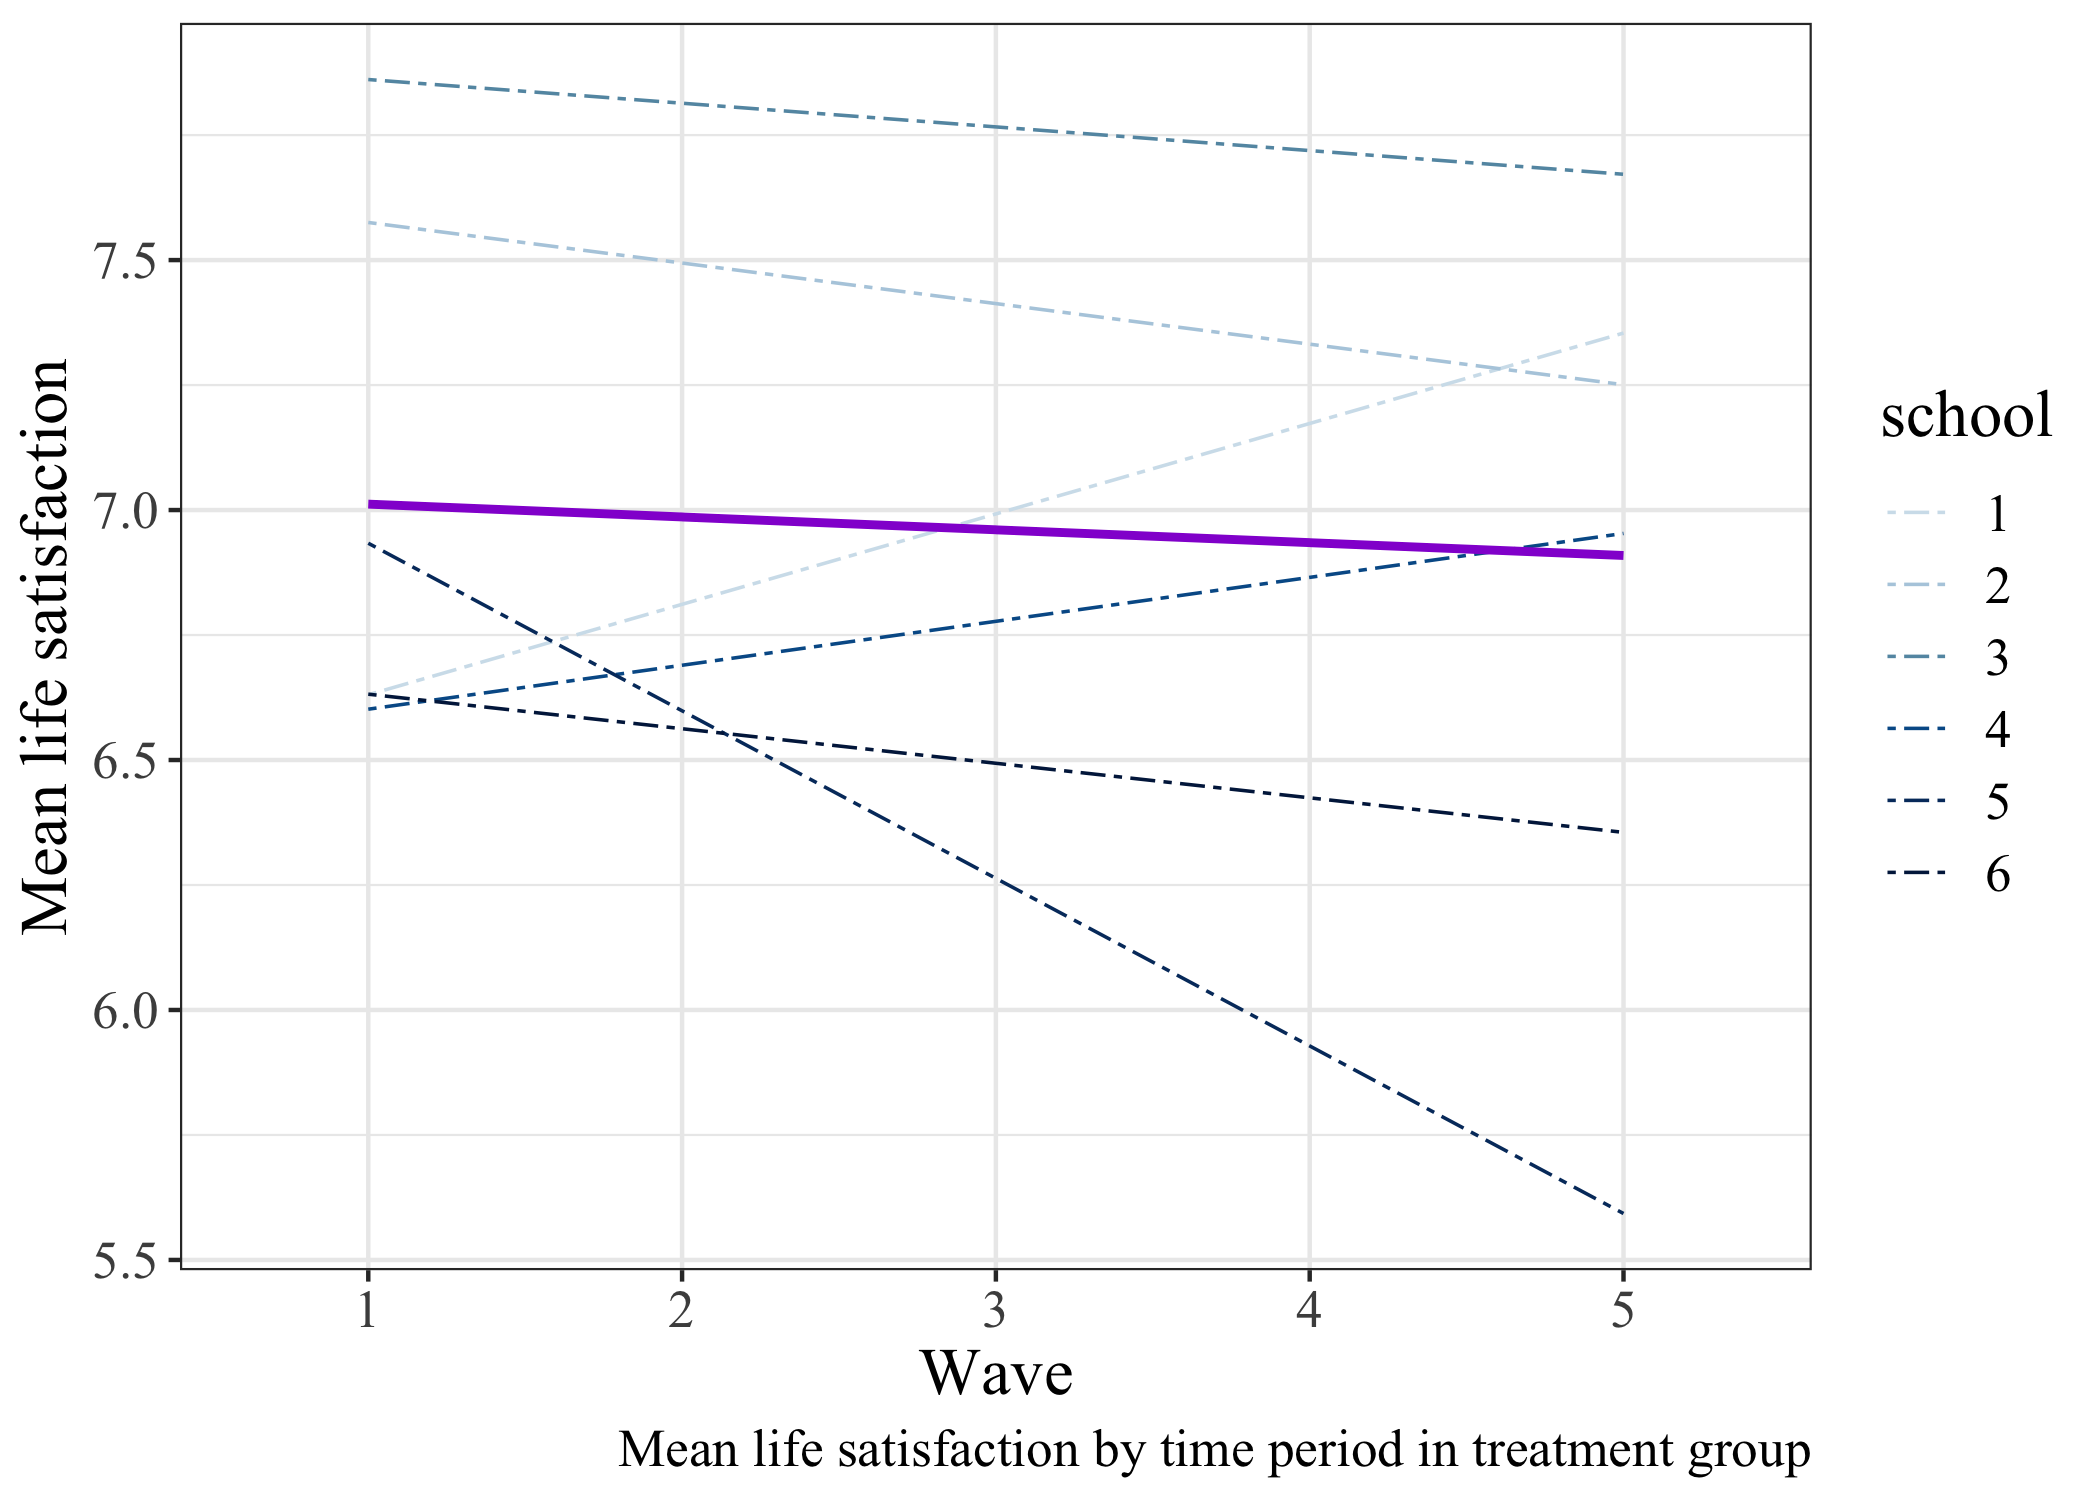
\includegraphics[width=0.8\linewidth,]{../figures/lsat_vs_time_by_school_treated} 

}

\caption{LS in treatment group}\label{fig:lsat-vs-time}
\end{figure}

Both approaches, no-pooling and complete pooling, have downsides for different reasons but they can be useful preliminary estimates, eventually leading up to what is known as partial pooling that comes out of a multilevel analysis. Therefore I will illustrate both the extremes, the complete pooling and the no-pooling approach in the following before I get to the details of partial pooling. The complete pooling and no-pooling model in comparison to the partial pooling model will be presented in a very simplified way. Life satisfaction will be explained with a varying-intercept model without any predictors. The purpose is to emphasize the characteristic features of the three approaches without unnecessary complexity in the model. In this example, \(\alpha\) and \(\sigma\) are given weakly informative priors and the models are estimated using rstanatrm functions `stan\_glm' abd `stan\_glmer'.

The simplest model is the pooled model, where life satisfaction is modeled as independent and identically distributed draws from a common distribution.
\begin{align*}
lsat_i & \sim {\mathrm {Normal}} (\alpha, \sigma) & \quad \text{for } i \in 1,...,n \\
\alpha & \sim {\sf Normal} (0, 10) \\
\sigma & \sim {\sf Exponential} (1)
\end{align*}
In the complete pooling approach, the population of schools is assumed to be invariant. This ignores the fact that schools are different and assigns the same intercept to each of the schools. If done like this, there is the risk of ignoring important variation in how schools correspond to the treatment (Mcelreath, 2020, p. 416). The total sample mean underfits the data, meaning that the model is insensitive to the details in the data and is learning too little from it. Ignoring the group-level variation is very likely misleading.

Whereas complete pooling ignores variation between schools, the no-pooling analyses overstates it and gives a different mean to each school:
\begin{align*}
lsat_i & \sim {\sf Normal} (\alpha_{j[i]}, \sigma) & \quad \text{for } i \in 1,...,n \\
\alpha_{j} & \sim {\sf Normal} (0, 10) & \quad \text{for } j \in 1,...,m,
\end{align*}
where \(j[i] \in 1,...,m\) is the school of student \(i\).
Although the \(\alpha_j\) are drawn from the same prior distribution, it has fixed parameters and thus no information is shared between observations in different schools. This makes the model very sensitive to the details in the data, you could say it is learning too much from it. The no-pooling approach includes the assumption that the schools are completely different and on school cannot tell anything about the other schools. This is equivalent to the variation among schools being infinite. But in reality, though schools are different in some ways, they are also very similar in in the way that each school helps to estimate the treatment effect in other schools. One should choose a model that incorporates the idea of learning from other groups while still accounting for systematic differences among the groups. This is exactly what partial pooling is attempting.

Partial pooling represents a compromise between the two extremes of excluding a categorical predictor from a model (complete pooling), or estimating separate models within each level of the categorical predictor (no pooling). For this simplified model with no predictors, the multilevel estimate for a given school \(j\) can be approciamted as a weighted average of the mean of the observations in the school (the unpooled estimate, \(\bar{y}_j\)) and the mean over all schools (the completely pooled estimate, \(\bar{y}_{\mathrm {all}}\)):
\begin{align*}
\hat{\alpha}_j^{\mathrm {multilevel}} \approx \frac {\frac{n_j}{\sigma_y^2}\bar y_j + \frac {1}{\sigma_{\alpha}^2}\bar y_{\mathrm {all}}}{\frac {n_j}{\sigma_y^2} + \frac {1}{\sigma_{\alpha}^2}}.
\end{align*}
In the partially pooled model, still each school has its own mean values but with the difference that now, these school-means share a prior which has its own parameters.
\begin{align*}
lsat_i & \sim {\sf Normal} (\alpha_{j[i]}, \sigma) & \quad \text{for } i \in 1,...,n \\
\alpha_{j} & \sim {\sf Normal} (\mu, \tau) & \quad \text{for } j \in 1,...,m
\end{align*} gelman hill p 253
We could also write the model with the school-level average in the mean equation for \(y\), and the \(\alpha_j\) values distributed around the country level average, \(\gamma\).
\begin{align*}
lsat_i & \sim {\sf Normal} (\alpha_{j[i]}, \sigma) & \quad \text{for } i \in 1,...,n \\
\alpha_{j} & \sim {\sf Normal} (\gamma, \tau) & \quad \text{for } j \in 1,...,m \\
\tau & \sim {\sf Exponentional(1)}
\end{align*}

After fitting the above models, I extracted the estimates of each of them and plotted them in @(fig:compare-models). (\url{https://jrnold.github.io/bayesian_notes/multilevel-models.html})

\begin{figure}[H]

{\centering 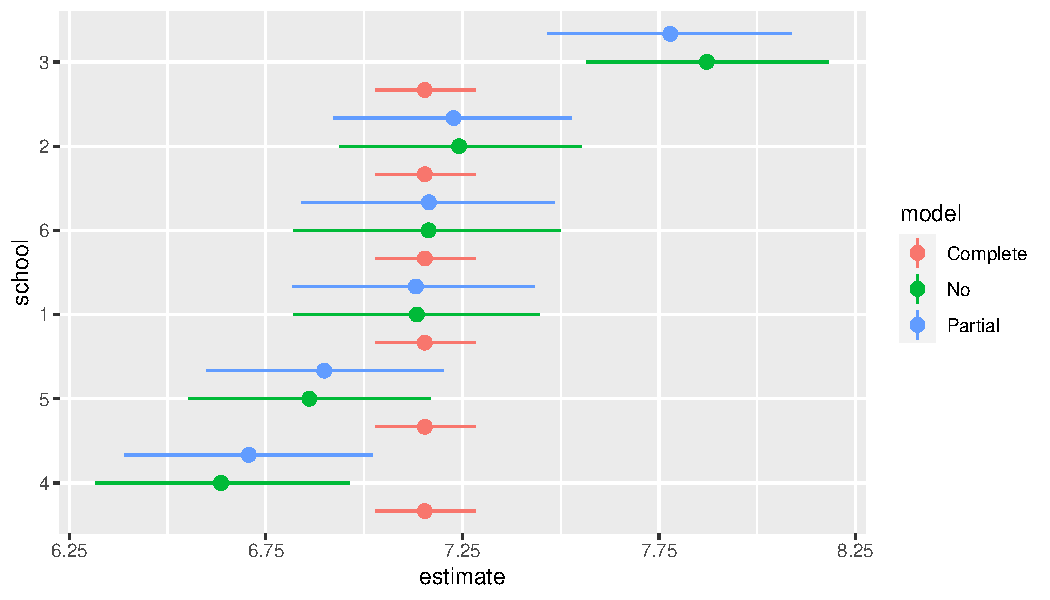
\includegraphics[width=0.8\linewidth,]{../figures/compare_models} 

}

\caption{Mean}\label{fig:compare-models}
\end{figure}

It shows clearly that when partially pooling information, both similarities and differences among groups are comprised. Partial pooling uses all the data available to perform inference for groups instead of just using local information which is especially useful when there is only a small number of observations in each group. The group estimates are supported to the extend of the whole data set and are not being limited to the number of observations per group. These estimates are less underfit than the grand mean and less overfit than the no-pooling estimates. As a consequence they tend to be better estimates of the true per-school means (mcelreath p423). Visually, this is shown by the blue dots (partial pooling), always being somewhere between the no-pooling estimates and the partial pooling estimates, being pulled towards the grand mean. The difference between the classical no-pooling estimates and the results from partial pooling is not very drastic. This is probably because the group-level variation is relatively small and that makes the multilevel model reduce to a classical regression with no group indicators. Also, the number of groups (6) is quite small which might be a reason why group-level variation cannot be estimated accurately. Still, it is worth the effort of expanding a classical regression in this way when adding the third level for the time periods later in the estimation. Generally, partial pooling will be especially helpful when there are only few observations in one school because then the no-pooling estimate will be overfit significantly. The difference between no-pooling and partial pooling becomes smaller, the more observations there are per cluster. The partial pooling produces noticeably better estimates and therefore will be used for my estimation. There are different tools to create a model that partially pooles information. I chose a Bayesian framework for my analysis since multilevel models, models with multiple levels of uncertainty, each feeding into the next, have natural Bayesian representation (elreath,14) (Gelman \& Hill p143). Also, in the context of the observed study, a multilevel model works extremely well because of several reasons (elreath 15):
* Adjusting estimates for repeat sampling - having more than one observation arising from the same student, a traditional, single-level model may be misleading
* Adjusting for imbalance in sampling - some students are sampled more than others, again, a single-level model could be misleading in this case
* Studying variation - I am interested in the variation of the treatment effect among schools. Multilevel models are of big help in this case because the model variation explicitly.

\hypertarget{bayesian-inference}{%
\subsection{Bayesian inference}\label{bayesian-inference}}

\emph{``Bayesian inference is the process of fitting a probability model to a set of data and summarizing the results by a probability distribution on the parameters of the model and on unobserved quantities such as predictions of new observations''} (gelman etal p1)
To set up what will follow in the next chapter about the explicit estimation, general terms from Bayesian inference are explained and formally written down. The notation comes from Gelman etal(chapter 1).
Unobservable vector quantities of population parameters of interest are denoted by \(\theta\), \(y\) is referred to as the observed data, the life satisfaction so to speak, and \(\tilde{y}\) are the unknown quantities (the potential quantities one will observe tomorrow - predictions). Bayesian statistical conclusions about a parameter \(\theta\), or unobserved data \(\tilde{y}\) are not made as specifying point estimates but they are made in terms of probability statements, expressed as \(p(\theta|y)\) or \(p(\tilde y|y)\) to show that these probability statements are conditional on the observed values of \(y\).
To make a probability statement about \(\theta\) given \(y\), a joint probability distribution for \(\theta\) and \(y\) is needed. The joint probability function is the product of two densities: the prior distribution \(p(\theta)\) and the sampling distribution \(p(y|\theta)\). Applying Bayes' rule yields the posterior density \(p(\theta|y)=\frac{p(\theta,y)}{p(y)}=\frac{p(\theta)p(y|\theta)}{p()y}\),
where \(p(y)=\sum_\theta{p(\theta)p(y|\theta)}\), and the sum is over all possible values of \(\theta\) (or \(p(y)=\int p(\theta)p(y|\theta)d\theta\) in the case of continuous \(\theta\)).
To make predictive inferences, a similar logic is applied:
The distribution of the unknown but observable \(y\) is
\[p(y)=\int p(y,\theta)d\theta=\int p(\theta)p(y|\theta)d\theta\], which is referred to as the prior predictive distribution. It is not conditional on previous observations of the process, and it is a distribution of some observable quantity.
From the same process, \(\tilde{y}\) can be predicted after observing the data \(y\).
The distribution of \(\tilde{y}\), for example of future measurements, is called the posterior predictive distribution. It describes a prediction for an observable \(\tilde{y}\) conditional on the observed \(y\):
\[p(\tilde{y}|y)=\int p(\tilde{y},\theta|y)d\theta \\
= \int p(\tilde{y}|\theta,y)p(\theta|y)d\theta \\
= \int p(\tilde{y}|\theta)p(\theta|y)d\theta.\]
The equations express the posterior predictive distribution as an average of the conditional predictions over the posterior distribution of \(\theta\). Given \(\theta\), \(y\) and \(\tilde{y}\) are assumed to be conditional independent.
Having decided on a specific probability model, the data \(y\) affect the posterior inference \emph{only} through \(p(y|\theta)\), the likelihood function.
Bayesian inference refers to statistical procedures that model unknown parameters (and also missing and latent data) as random variables. It starts with a prior distribution (more on that point in Section \ref{subsec:priors} on the unknown parameters and updates this with the likelihood of the data, yielding a posterior distribution which is used for inferences and predictions (gelman and hill p143) (To my proof reading boyfriend: wie könnte man den Absatz schön umformulieren?)

\clearpage

\hypertarget{estimation}{%
\section{Estimation}\label{estimation}}

\label{ch:estimation}
For model estimation I decided to use the `brms' package by Bürkner (Bürkner (2017)). It implements Bayesian multilevel models in `R' using the probabilistic programming language `Stan'. It allows for individual prior specifications and facilitates incorporating prior distributions that reflect the users' beliefs. The package is also suitable for assessing and comparing models with the Watanabe-Akaike information criterion and leave-one-out cross-validation.

\hypertarget{the-model}{%
\subsection{The model}\label{the-model}}

\label{sec:model}
As mentioned above, the intervention under study is not a fully randomized experiment. To address the issue of potential differences between students from the control group and students from the treatment group, , I use difference-in-difference regressions to estimate the effect of additional music lessons on pupils' life satisfaction and three areas of satisfaction are also observed as a outcome variable. Using this method, systematic pre-treatment differences are no longer a threat to identification. There is the underlying common trend assumption that requires that if the treatment were not undertaken, both the control group and the treatment group would have experienced the same time trend.
The model I am using to fit the data includes varying intercepts on the school level and on the student level and varying slopes for each school. This assumes that schools have similar features but also, the way the treatment was introduced in each class might have differed slightly in each school. The individual intercept for each student is included to account for any unobserved background characteristics. The model, including the structure of the model and the distribution of the hyper-parameters is as follows:

\begin{align*}
lsat & \sim {\sf Normal} (\mu_{ijt}, \sigma), \\
\mu_{ijt} & = \beta_0 + \beta_{1j[i]} T_i + \sum\limits_{l=2}^5\delta_{lj[i]} (T_{i} \times \text{Period}_{t}) + \lambda_t + \mu_{j[i]} + \alpha_{i} + \epsilon_{ijt}, \\
\beta_0 & \sim  {\sf Normal}(7,2), \\
Population-level effects & \sim {\sf Normal}(0,5), \\
Group-level effects & \sim {\sf Cauchy}(0,1), \\
\sigma & \sim {\sf Exponential}(0,5)
\end{align*}

The study of effectiveness of the music project, with the students in school \(j\) having a certain unknown parameter vector \(\theta_j\), it might be reasonable to expect that estimates \(\theta_j\), which represent a sample of schools, should be related to each other. This is achieved in a natural way by using a prior distribution in which life satisfaction is viewed as a sample from a common \emph{population distribution}. A key feature of such applications is that the observed data, \(y_{ij}\), with student index \(i\) within group indexed by \(j\), can be used to estimate aspects of the population distribution of the \(theta_j\)'s even though the values of \(\theta_j\) are not themselves observed. In contrast, hierarchical models can have enough parameters to fit the model well, while using a population distribution to structure some dependence into the parameters, thereby avoiding problems of overfitting.

I simultaneously investigate the treatment in six different schools. The analysis is restricted to wave 1 (pre treatment) and wave 2 (post treatment). The regression equation is:

The hierarchical structure in my model looks as follows:

where

\begin{itemize}
\tightlist
\item
  \(y_{ijt}\) is the outcome of pupil \(i\) in school \(j\) at time \(t\).
\item
  \(T_{i}\) is a binary indicator of whether or not pupil \(i\) is in the treatment group. We model a fixed effect for the treatment group because the treatment takes place at the aggregate level (class). Therefore, bias in the estimate of the treatment effect may results from unobserved factors at the class level.
\item
  \(\delta_{l2j[i]}\) is the treatment effect in wave \(l\). The effect is allowed to vary across schools.
\item
  \(\lambda_t\) denotes period fixed effects.
\item
  \(\alpha_{i}\) models individual-specific unobserved factors. Individual heterogeneity is model because we have repeated observations for the same pupils over time.
\item
  \(\epsilon_{it}\) is an error term.
\end{itemize}

(Simulation?)

For doing \emph{blah} I use \emph{blub} {[}ref{]}

\hypertarget{prior-distribution}{%
\subsection{Prior distribution}\label{prior-distribution}}

\label{sec:priors}
As stated above in @ref\{sec:methodology\} in a Bayesian framework parameters are not point estimates but they have distributions. The specification for these parameters are called prior distribution because they must be specified \emph{before} the model is fit to data and it assigns them a probability to every possible value of each parameter to be estimated. If the specification is done properly, for all parameters in the model, a Bayesian model yields a joint prior distribution on parameters and data, and hence a prior marginal distribution for the data (Gabry p5). This process can be described as the prior distributions and data interacting to finally produce the posterior distribution. The posterior can be seen as a compromise between the prior distribution and the likelihood function. Therefore, the choice of the prior should be done carefully since it can determine the outcome severely. After identifying the type of data being described, creating a descriptive model with meaningful parameters, and defining a likelihood function, the next step is to establish a prior distribution over the parameter values (kruschke 110). The prior distribution indicates the believes about the distribution of each parameter without knowing the specific data. Depending on the choice of prior and the respective data set, the ``compromise'' favors one of them over the other. Flat priors or super-vague priors (\(\sf {N}(0,1e6)\)) are usually not recommended. They lead to a posterior distribution that is mainly influenced by the data which means that though the data set is very well described by the model, predictions are very poor. The model only ``learned'' about the distribution from the data because the prior did not carry any information. However if the prior has strong believes about the distribution of the parameters, meaning the prior distribution is sharply peaked, and there are only relatively few data, the posterior distribution is more influenced by the prior. Generally, weakly informative priors (\(\sf{N}(0,10)\)) are recommended because they help by providing a very gentle nudge towards reasonable values of the parameter (mcelreath p 299). If there is a reasonable large amount of data, they will dominate while the prior becomes less important. In case of not very meaningful data though, the ``weakly informative prior'' make up for it by strongly influencing the posterior inference. This relation is illustrated in @ref\{fig:flat-peaked\}. The upper row shows the posterior that appears when having a prior distribution \(lsat \sim {\sf Normal}(5, 200)\). The standard deviation in this prior is huge and gives barely any useful information about the distribution of life satisfaction among the population. The shape of the posterior is almost identical to the one of the likelihood. The opposite is the case when the prior is highly informative. A normal distribution with parameters of \(\mu = 5\) and \(\sigma = 1\) suggests that life satisfaction is very narrow around the mean of 5. The prior is so sharp that the posterior distribution is noticeably influenced by the prior. Bayesian models with proper priors are generative models (Gabry p5)

\begin{figure}[H]

{\centering 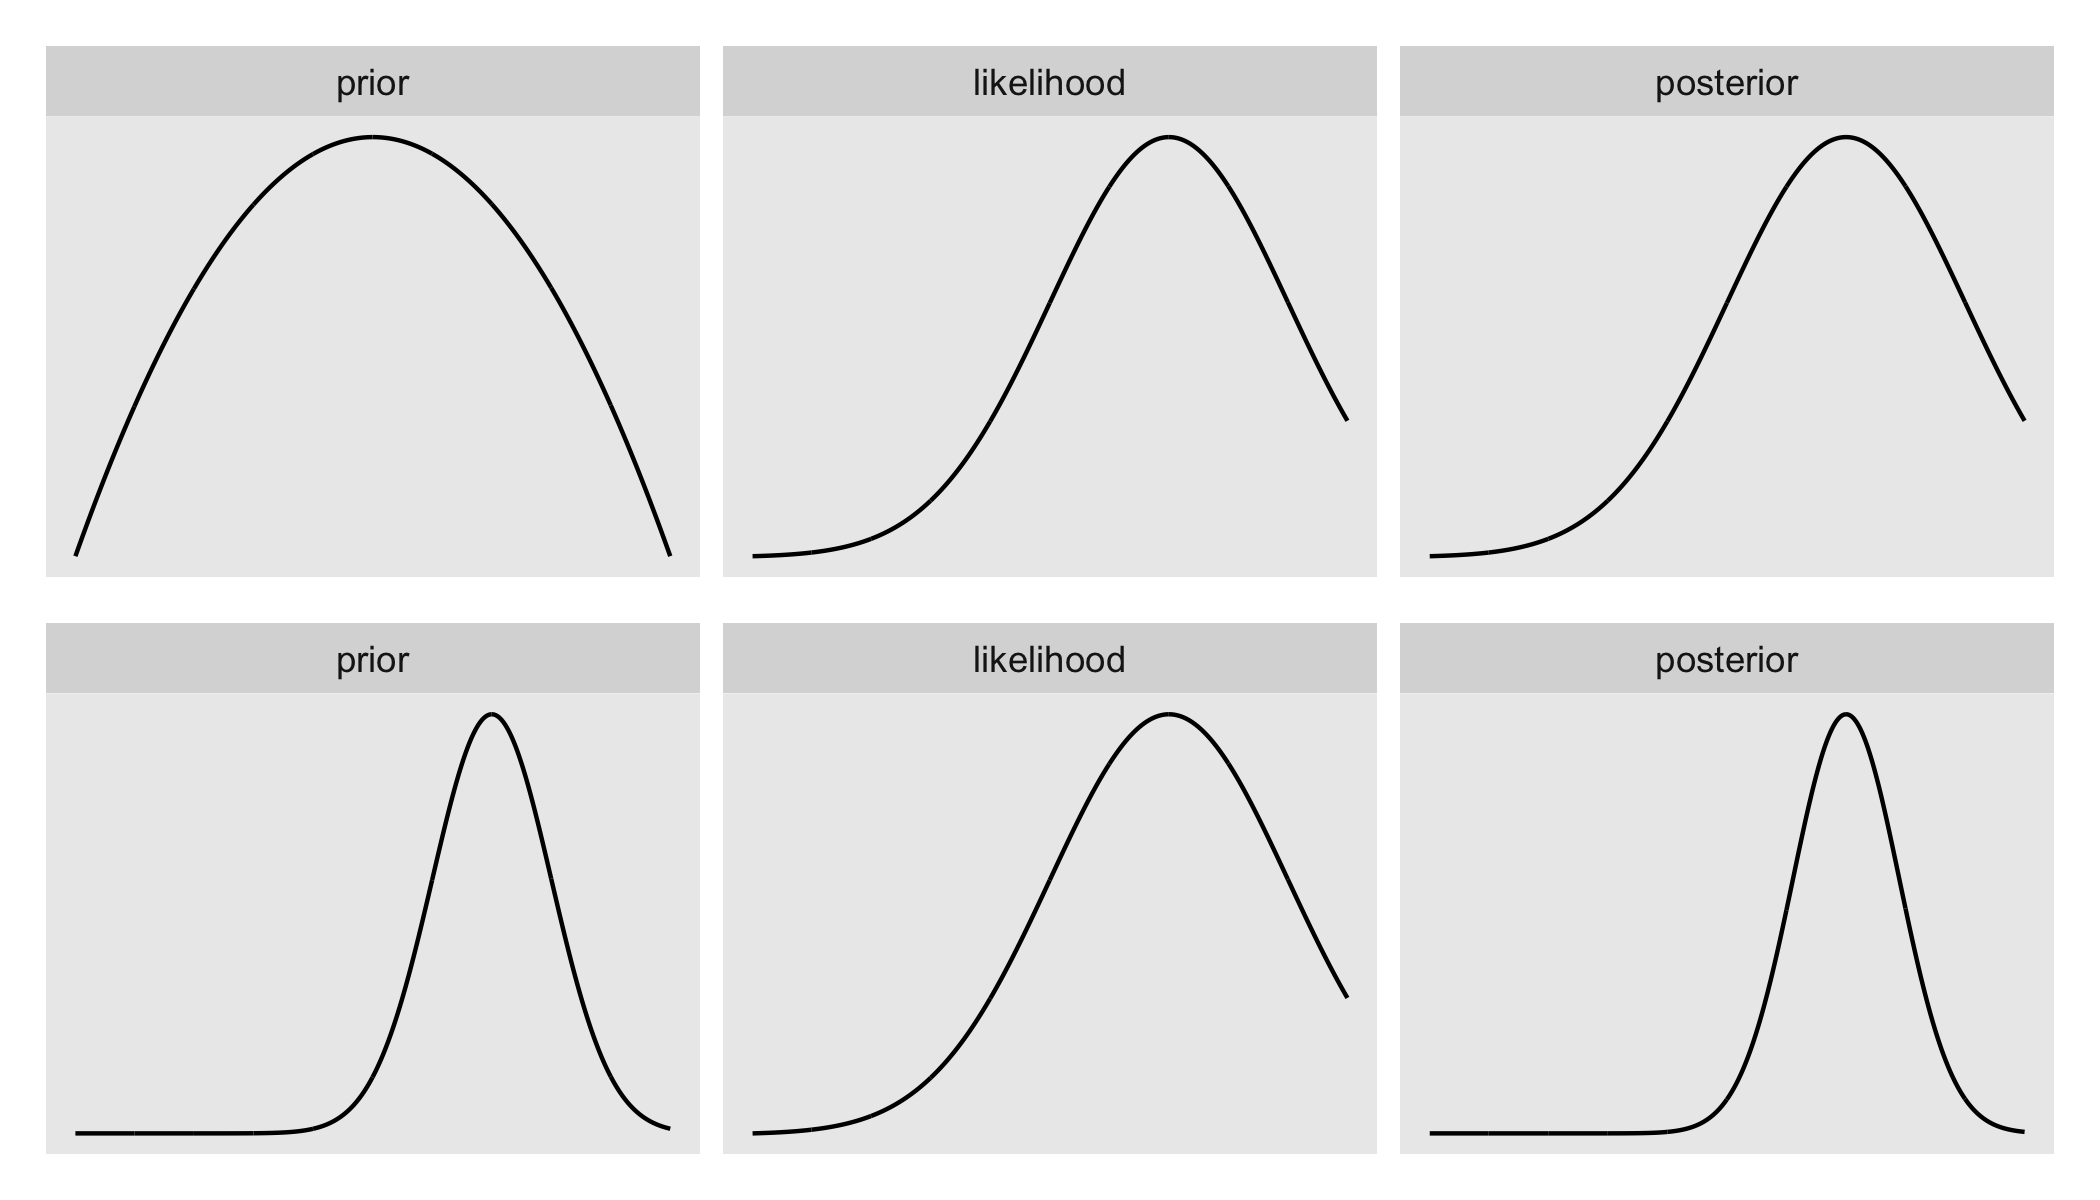
\includegraphics[width=0.8\linewidth,]{../figures/flat_peaked} 

}

\caption{Flat vs peaked prior}\label{fig:flat-peaked}
\end{figure}

A good prior also tackles the problem of overfitting which was discussed above. By choosing a skeptical prior. The term skeptical refers to the prior being skeptical about values outside the range of parameter values that are not reasonable. The most common skeptical prior is the regularizing prior which effectively reduces overfitting whil still allowing the model to learn about the regular features of a sample.
To decide on proper priors, I plottet the influence of different priors on the distribution of the outcome variable, life satisfaction. This helped me deciding on priors that influenced the oucome in a way that the largest part of the distribution was on a reasonable scale while extreme values are still possible. To begin with, the prior for the estimate is \(N(7,2)\) (Figure\ldots). Life satisfaction as it is measured in this setting spreads on a range from 0 to 10 with most of the responses in the upper third. For the standard deviation I chose \(\sf {Exp}(0.5)\) which is wide enough for all values on the satisfaction scale to remain possible. For the population-level and group-level effects, I came to the conclusion that a weakly-informative prior of \(\sf {N}(0,1)\) is best. To show this, I plotted predicted values from different prior predictive distributions:

\begin{figure}[H]

{\centering 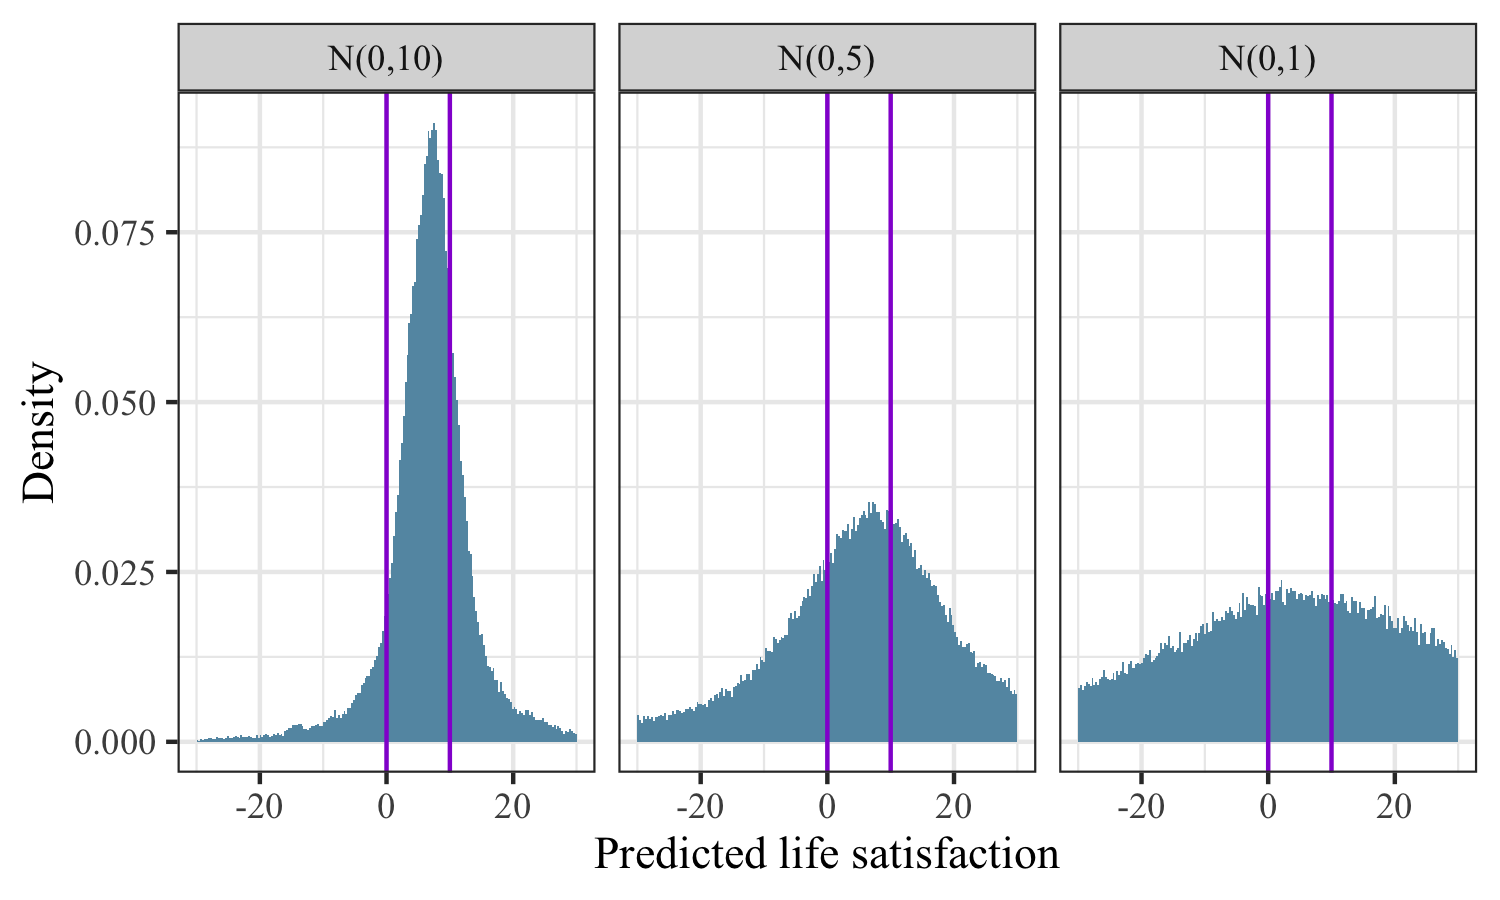
\includegraphics[width=0.8\linewidth,]{../figures/prior_predict} 

}

\caption{Prior predictive distribution}\label{fig:lsat-predicted}
\end{figure}

made some prior predictive simulations as suggested by MacElreath. This method is useful for understanding the implication of a prior and is neatly executed by Gabry ( see full code\ldots). It simulates predictions from a model, using only the prior distribution instead of the posterior distribution. Once priors are chosen, they imply a joint prior distribution of individual life satisfaction (elreath p85). This procedure is based on choosing priors conditional on pre-data knowledge of the data, on general facts so to say (elreath, p100). Only when this step is done, the model is applied to the data.

\begin{figure}[H]

{\centering 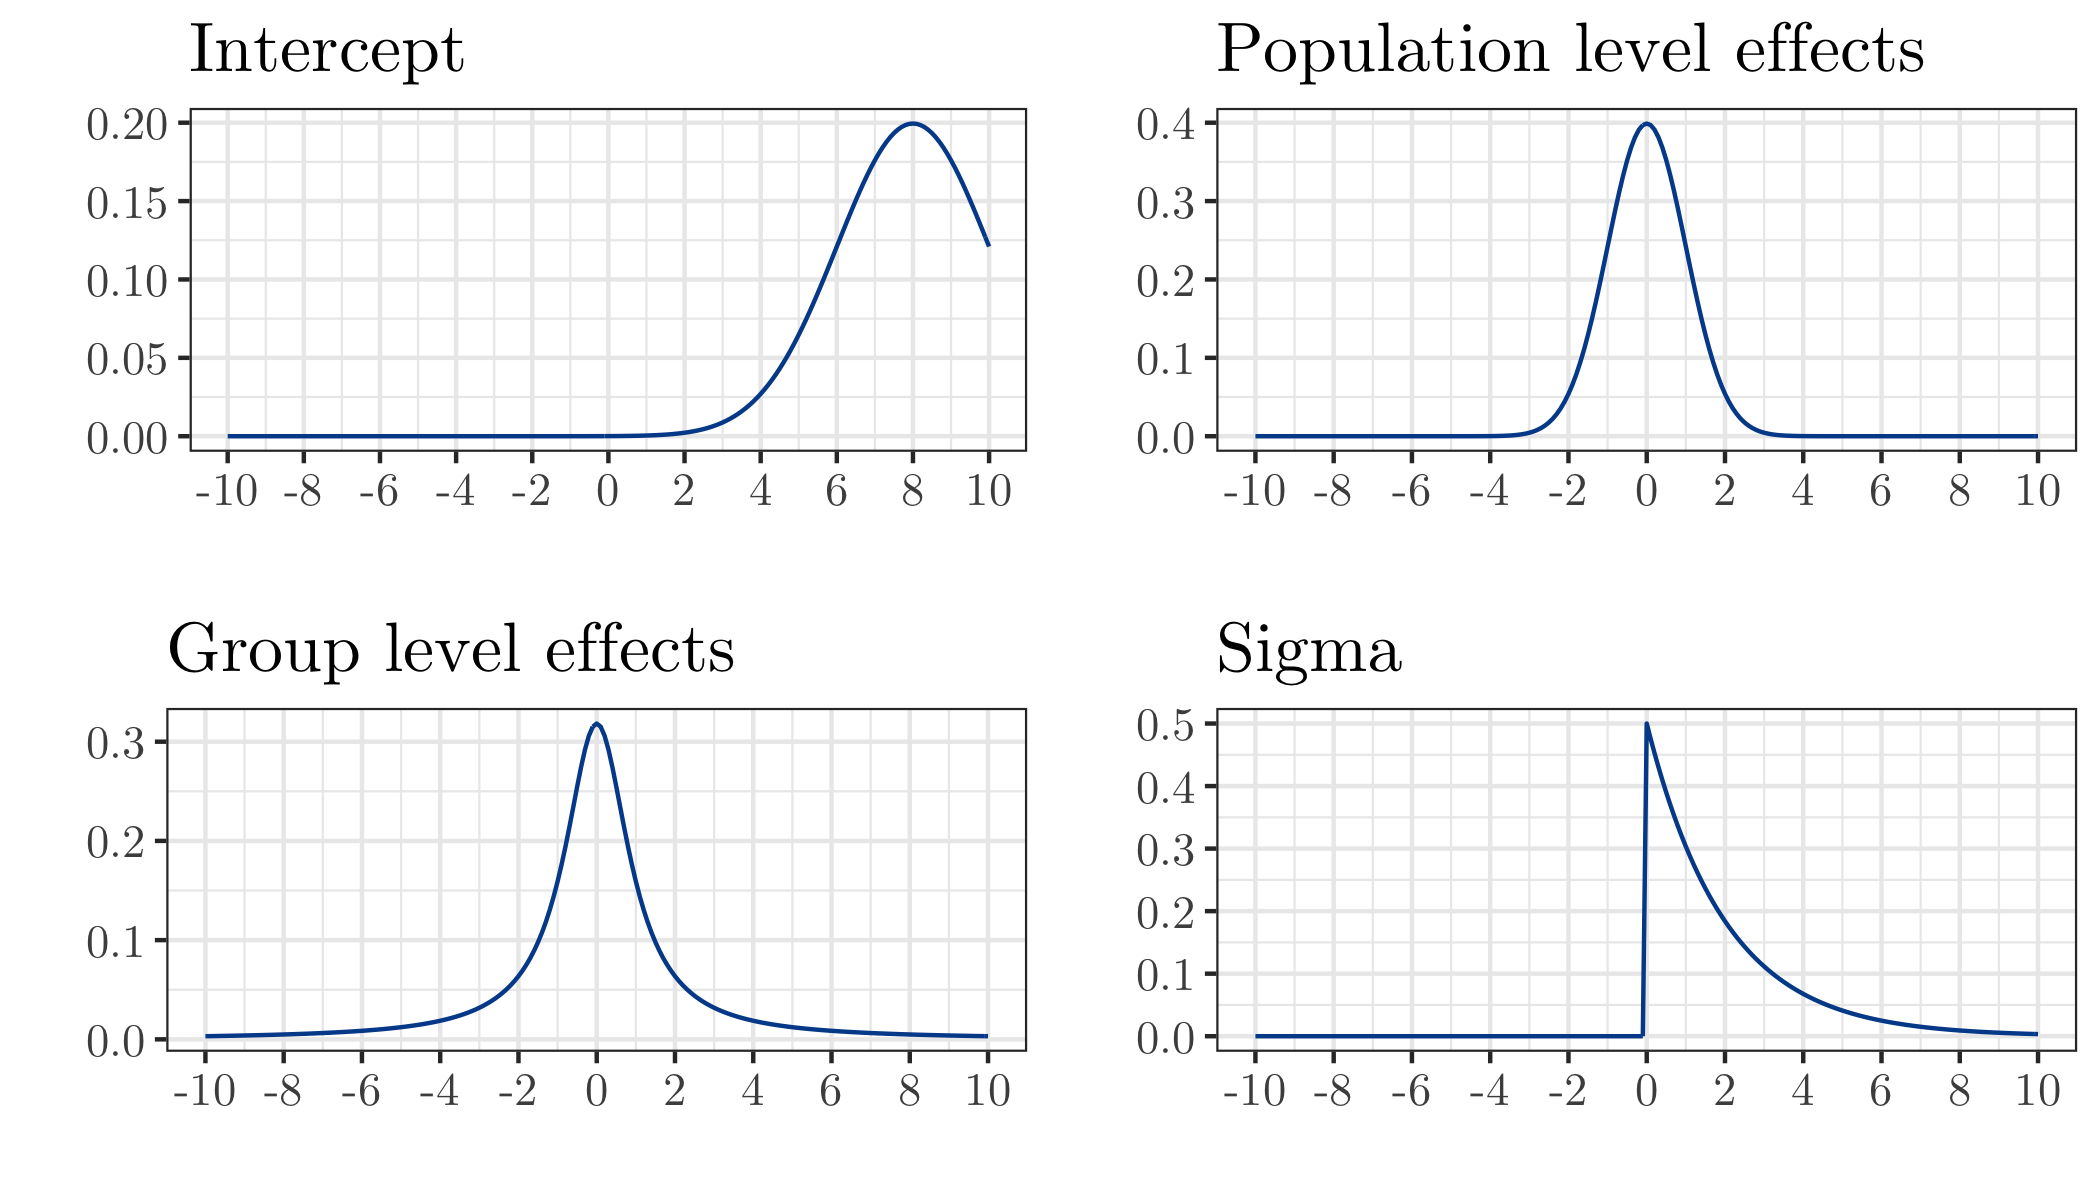
\includegraphics[width=0.8\linewidth,]{../figures/plot_priors} 

}

\caption{Plots of chosen priors}\label{fig:chosen-priors}
\end{figure}

The assumption of a normally distributed effect is hard to justify, considering the distribution of life satisfaction as it is in wave 1 (Figure \ref{hist-lsat}). The peaks for values of life satisfaction at 5 and at 10 do not really represent a normal distribution. The main reason for the use of normal distributions is mainly mathematical tractability. However, if the family of Bayesian models is inapporpriate, Bayesian answers can be quite misleading (Rubin (1981) 394)

\hypertarget{model-validation}{%
\subsection{Model validation}\label{model-validation}}

\label{sec:validation}
After fitting the model in the previous section, I will now check its fit to data. A basic approach to asses the models adequacy is what is described as ``phenomenological Bayesian monitoring'' in Rubin (1981) (394) also: Gelman Bayesian Data Analsis ch.~5.5. The method is as follows. The posterior distribution, the distribution of the model parameters conditional on the observed data, can be used to generate a posterior predictive distribution. The implied predictions come from sampling from the posterior distribution to simulate predictions. The idea behind this approach is then to compare the posterior predictive distribution to a) the actual data and b) scientific judgment about plausible values of such data. The idea behind this approach is that if the model fits well, there should not be any systematic differences between what the model predicts to what the real data show and they will not contradict with plausible values but will be typical of them. Again, I follow Gelmans notation (p 145) for more detailed description of the posterior predictive checking. The observed data are denoted as \(y\), \(\theta\) is the vector of parameters, including all the hyperparameters. The replicated data are defined as \(y^{\mathrm{rep}}\). Thinking predictively, these are data that would be observed in the future if the experiment were replicated with the same model and the same value of \(\theta\) that produced the observed data \(y\). The distribution of \(y^{\mathrm{rep}}\) given the stat of knowledge is the posterior predictive distribution:
\[p(y^{\mathrm{rep}}|y)=\int p(y^{\mathrm{rep}}|\theta)p(\theta|y)d\theta.\]
I chose a graphical representation of the PPCs. Instead of calculating posterior probability, simulated data are plotted, to be visually compared to observed data.
Figure \ref{fig:post-dens-overlay} shows the distribution of many replicated datasets drawn from the posterior predictive distribution (thin light lines) compared to the empirical distribution of the observed outcome (thick dark line). It shows that the assumption of a normal distribution might have been too strong. Therefor the model does not perform very well in capturing the observed skewness which is shown in Figure \ref{fig:post-skew}.

\begin{figure}[H]
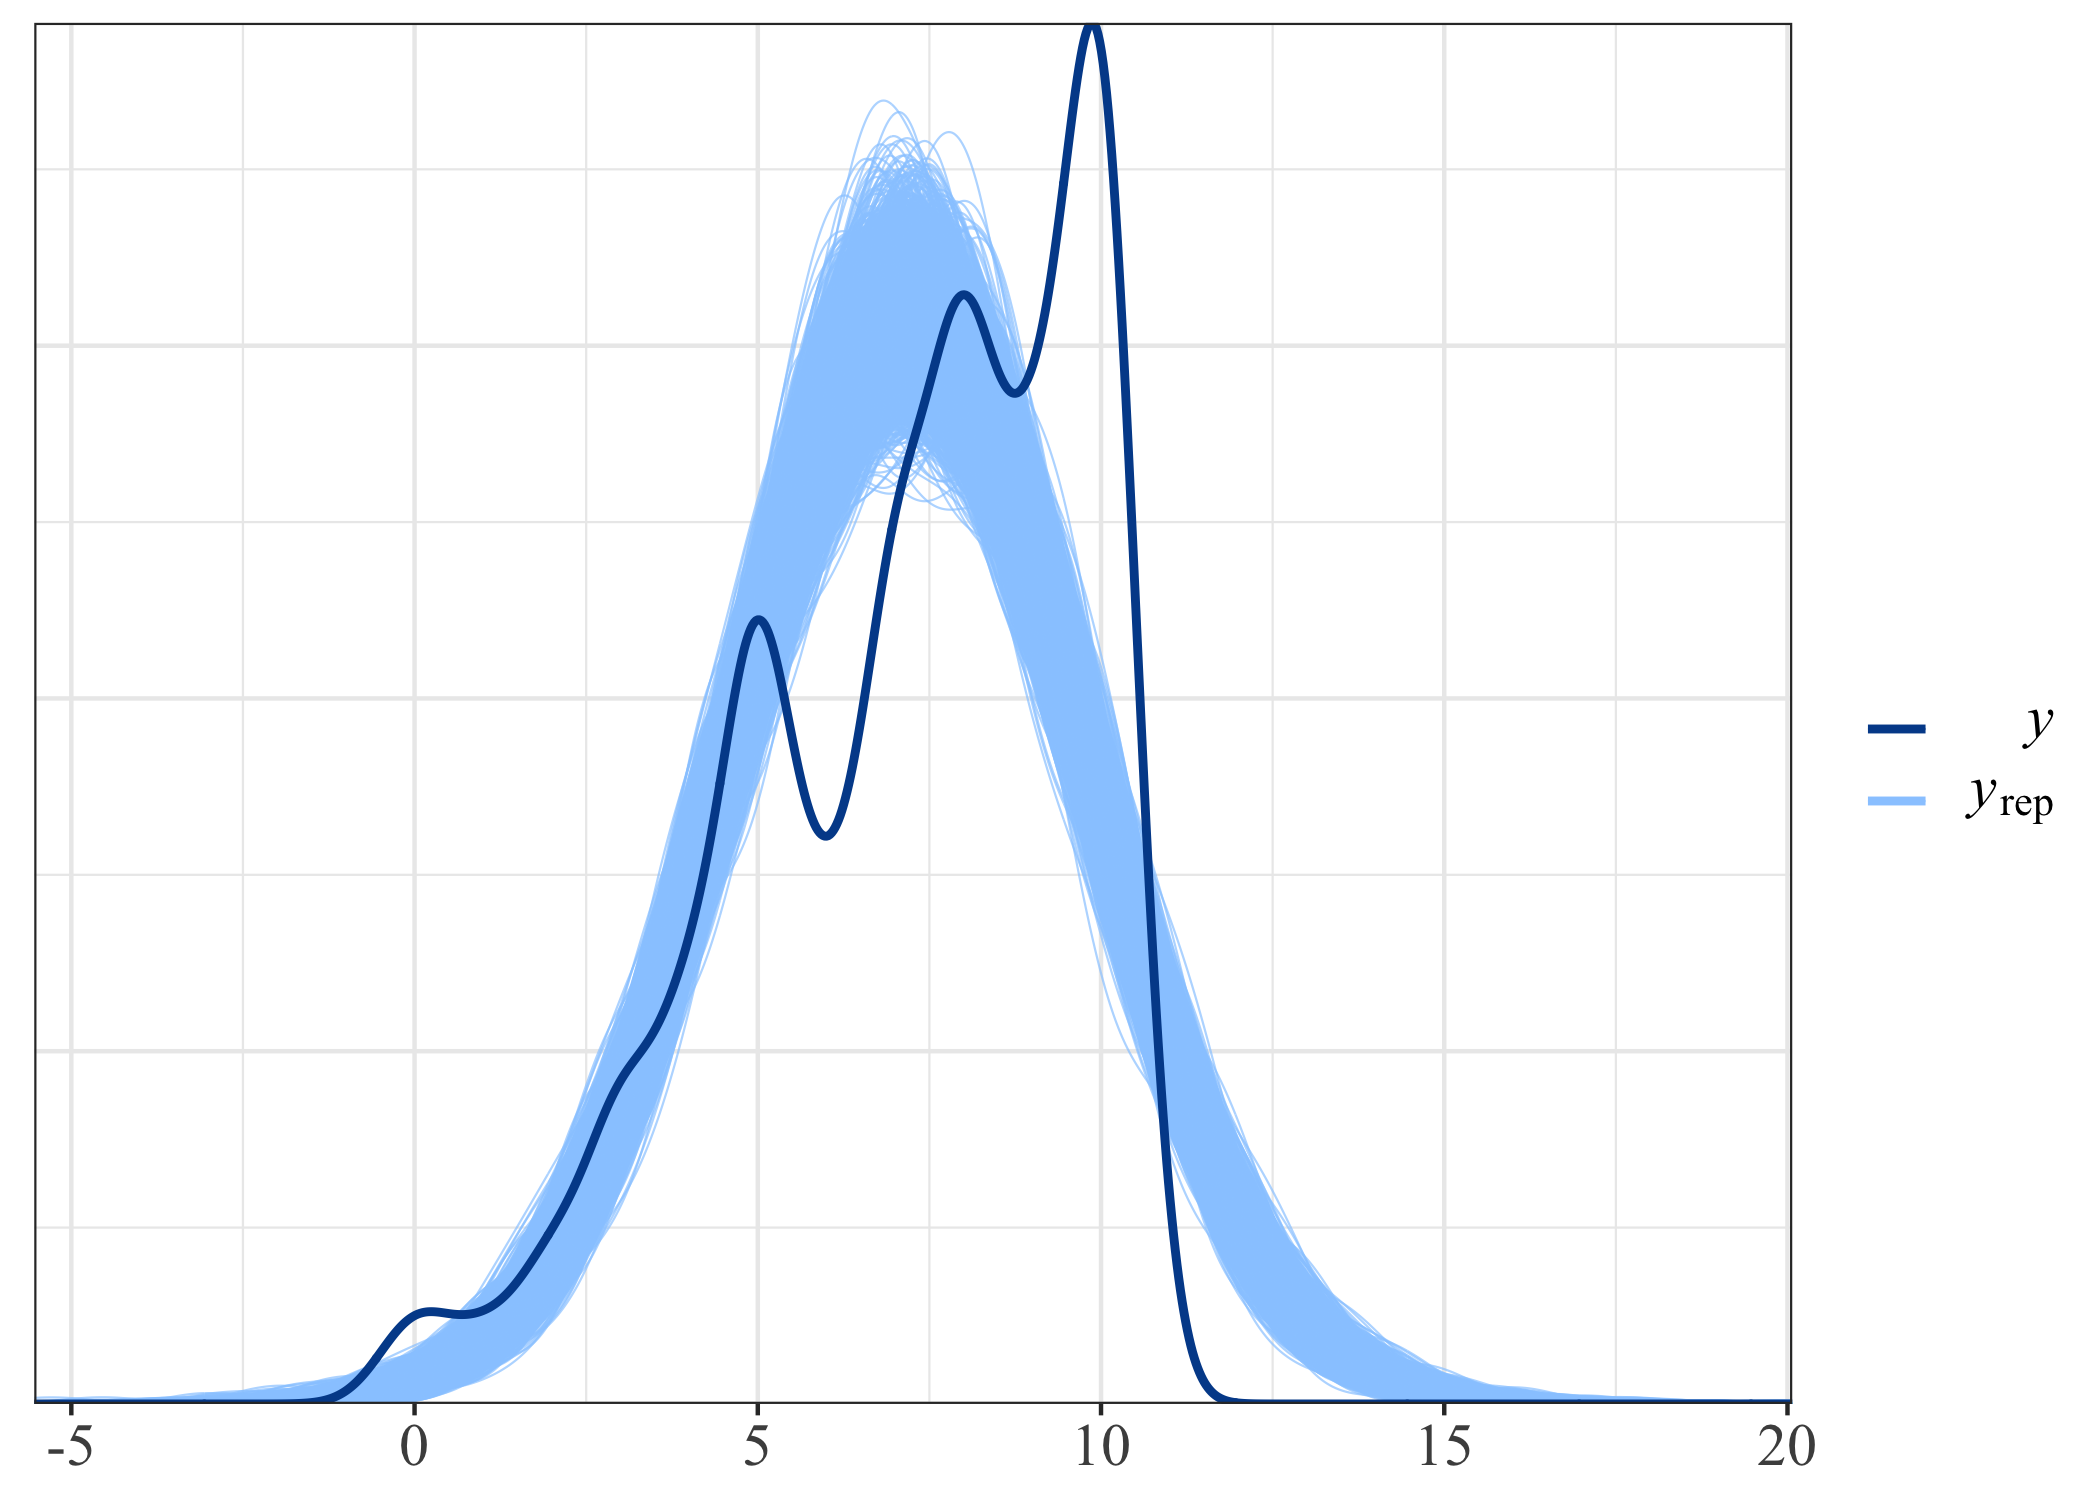
\includegraphics[width=0.5\linewidth,]{../figures/post_dens_overlay} 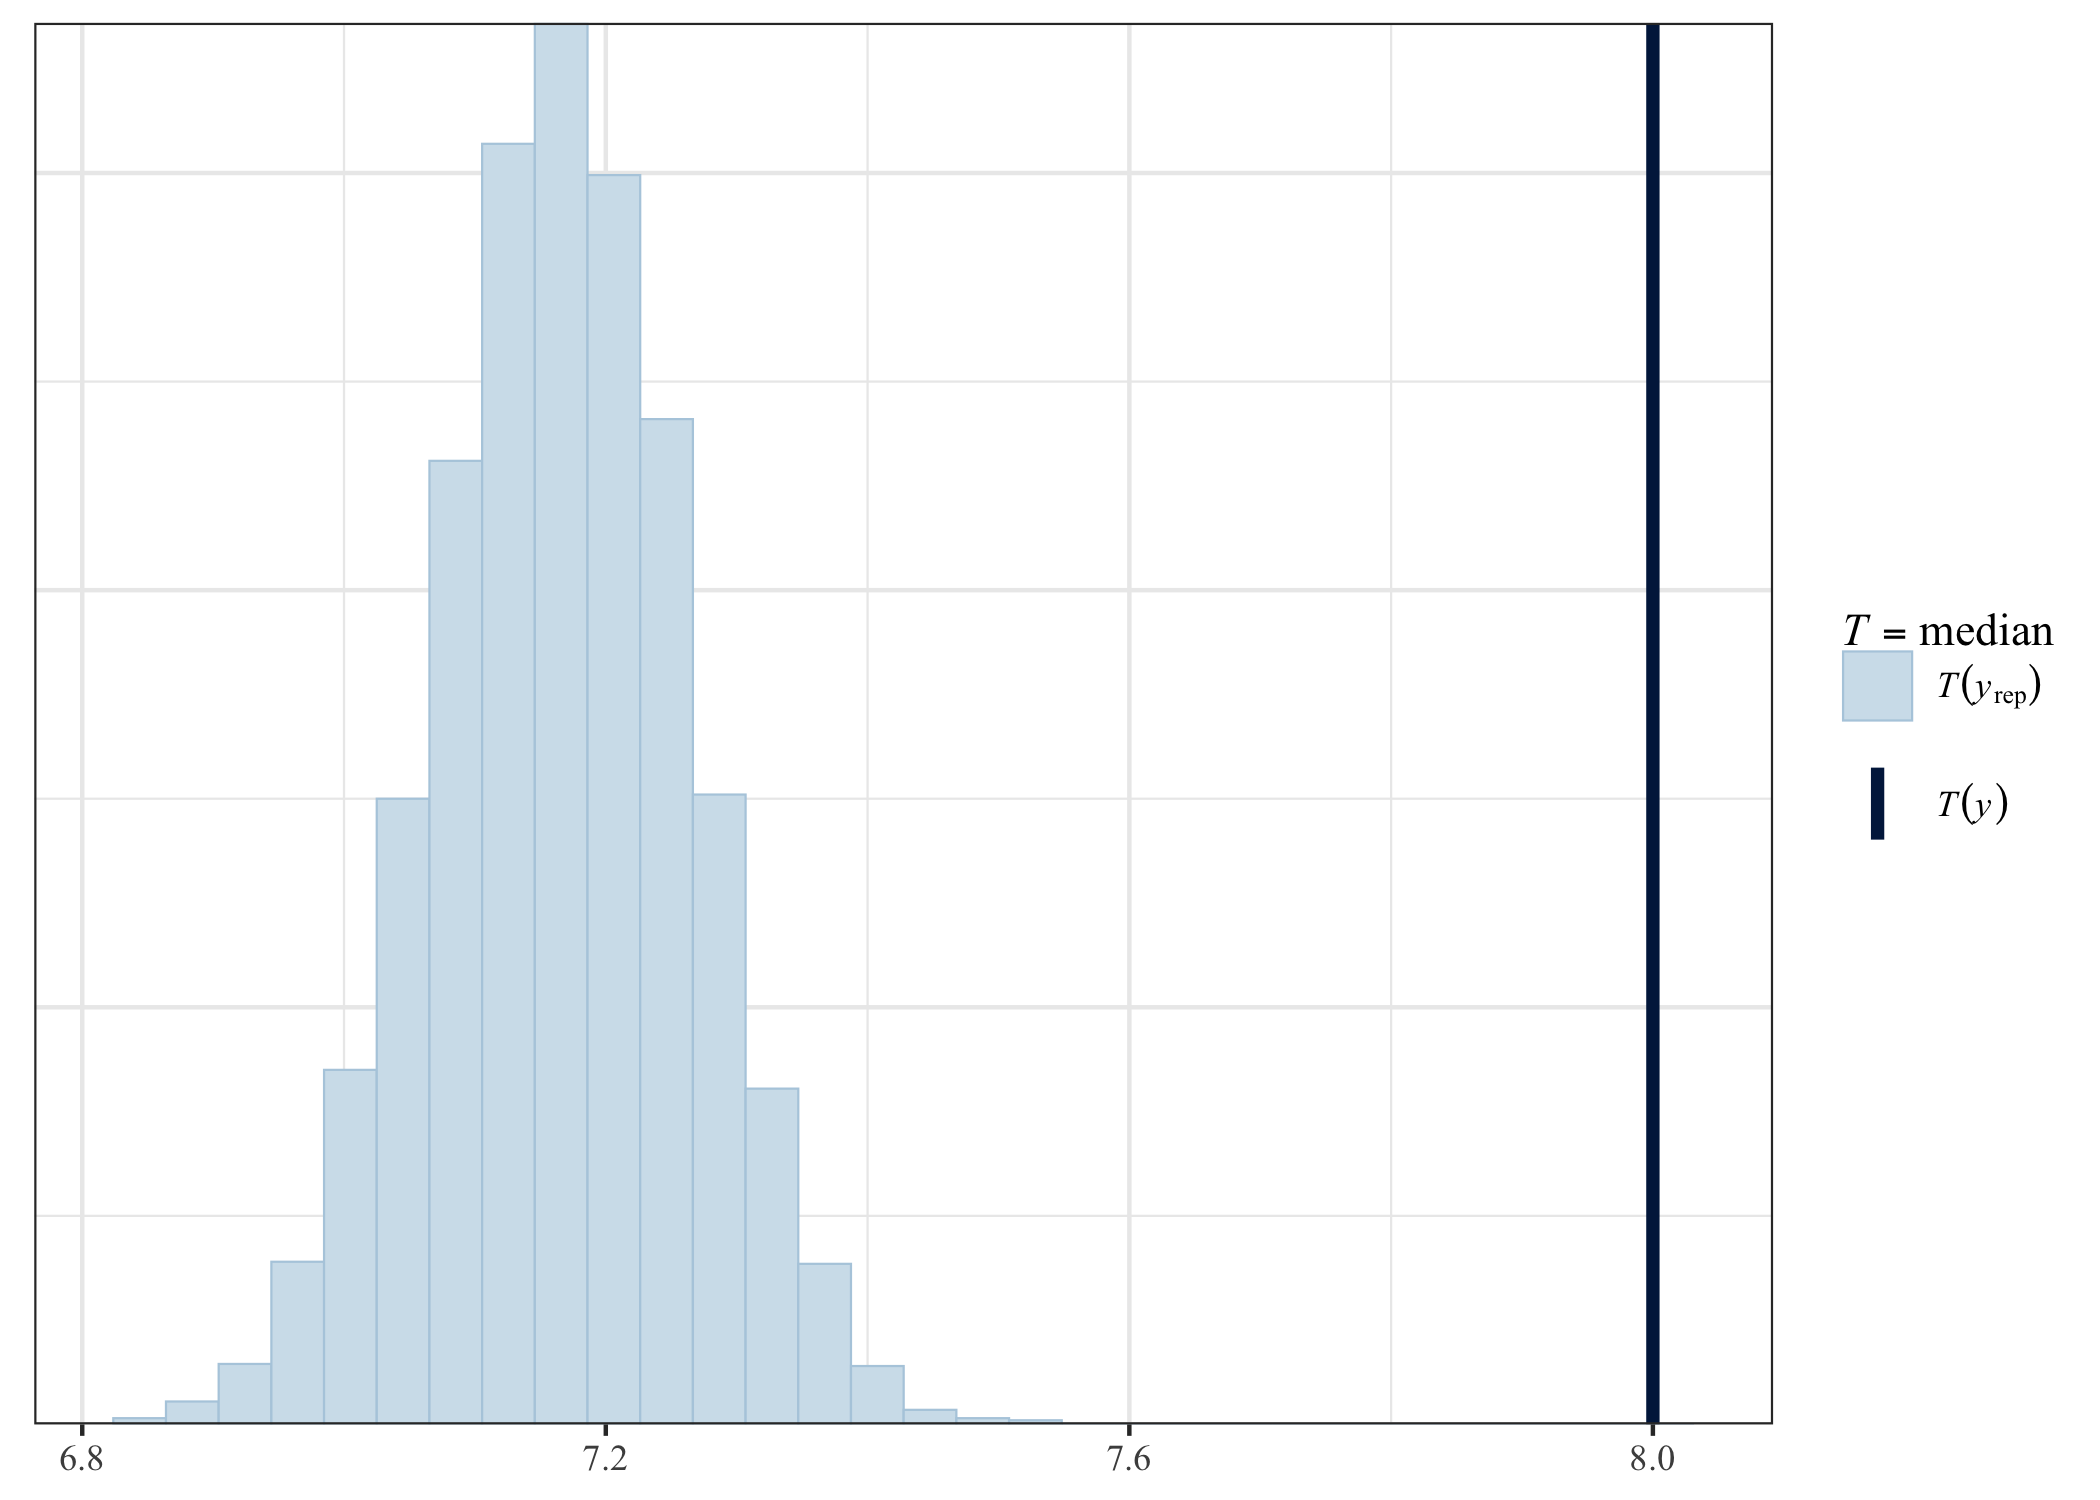
\includegraphics[width=0.5\linewidth,]{../figures/post_skew} \caption{Posterior predictive check}\label{fig:post-dens-overlay}
\end{figure}

Looking at the features of the data and the replicated data, which were not explicitly included in the model, indicates the need to extend or modify the model.

\clearpage

\hypertarget{results}{%
\section{Results}\label{results}}

\label{ch:results}
Below in Figure \ref{fig:m1-coef}, all of the parameter estimates from the MCMC draws are shown. It plots posterior intervals for the parameters where the thick lines are the 50\% intervals and the thinner outer lines the 90\% intervals. In this chapter I will focus on the explanation of treatment effects that can be observed in terms of life satisfaction. I will also bring in the results for the three areas of satisfaction for friends, class and school. Those results will be discussed in less detail, they serve to potentially suggest an explanation where the effects on life satisfaction stem from.

\begin{figure}[H]

{\centering 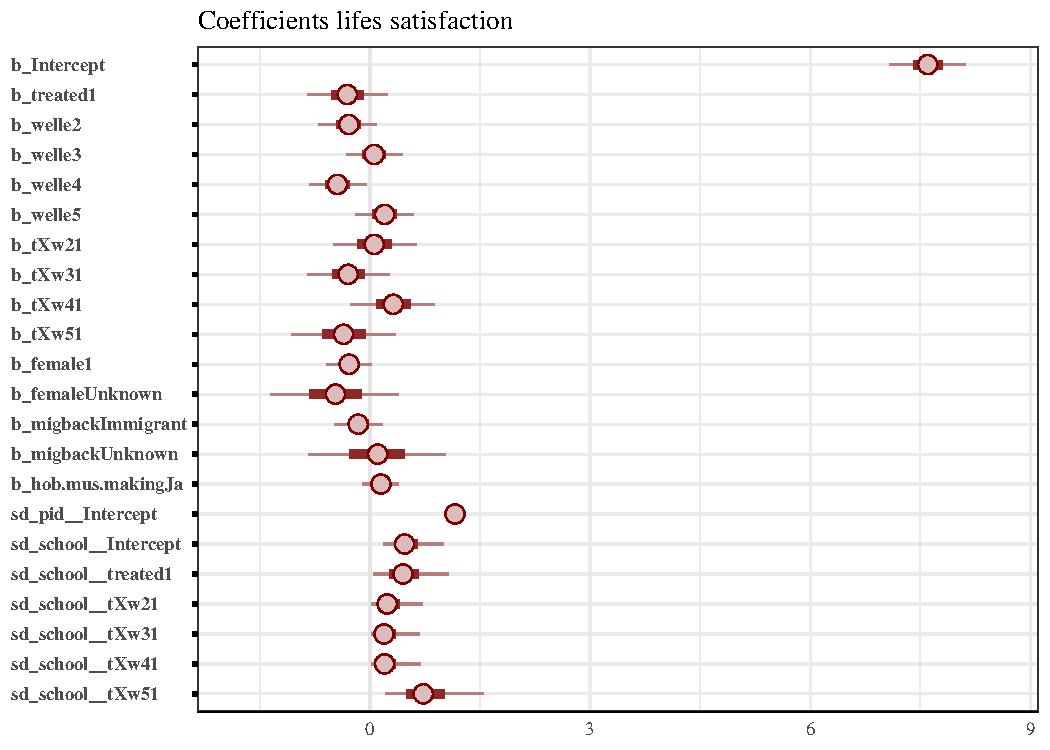
\includegraphics[width=0.8\linewidth,]{../figures/m1_coef} 

}

\caption{Parameter estimates}\label{fig:m1-coef}
\end{figure}

\hypertarget{life-satisfaction}{%
\subsection{Life satisfaction}\label{life-satisfaction}}

\label{sec:life-satisfaction}

\hypertarget{average-school}{%
\subsubsection{Average school}\label{average-school}}

Plotting life satisfaction throughout time for the treatment and the control group respectively gives the following picture:

\begin{figure}[H]

{\centering 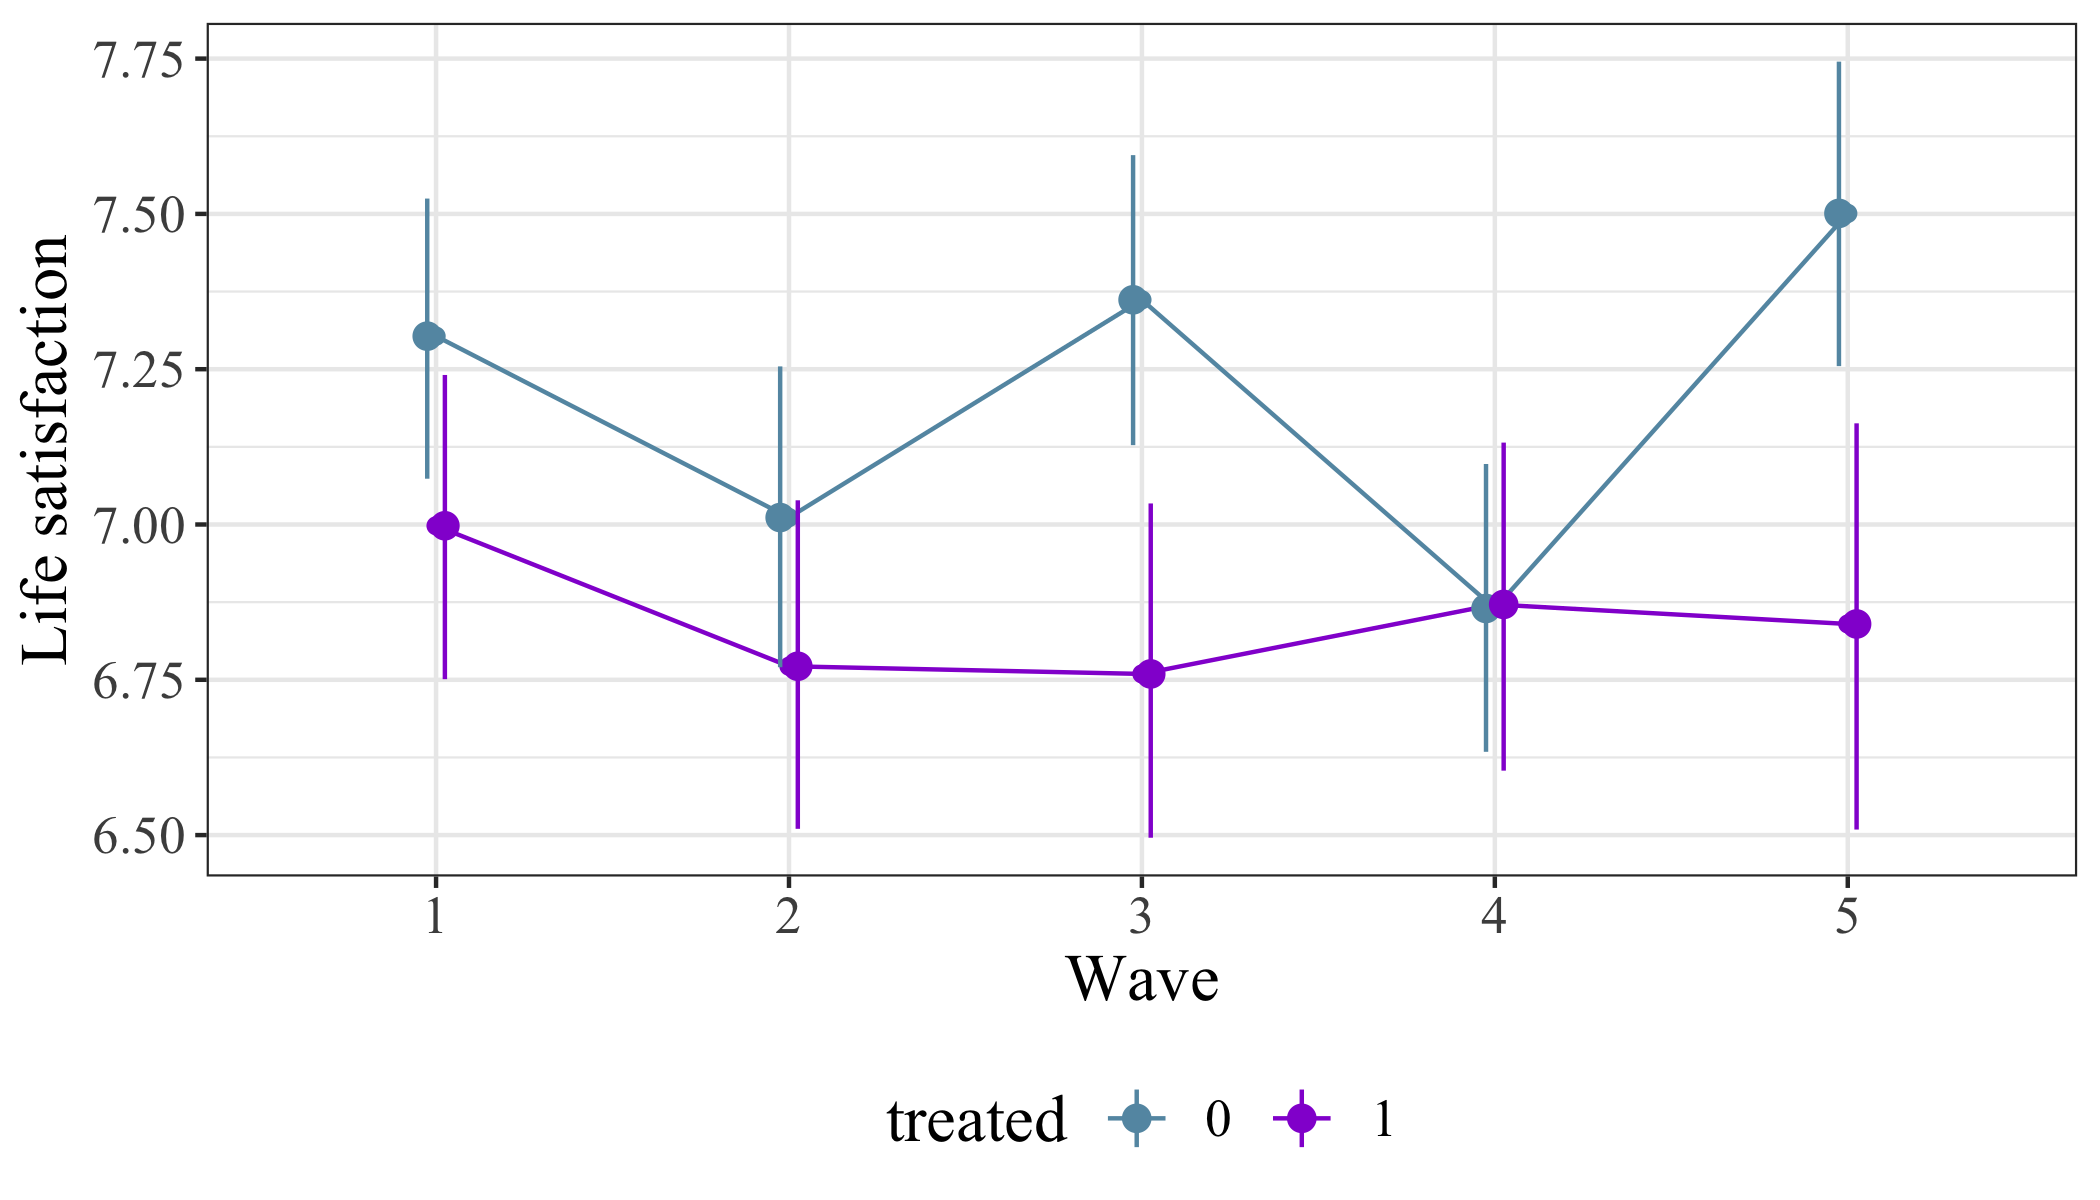
\includegraphics[width=0.8\linewidth,]{../figures/lsat_pred} 

}

\caption{Predicted life satisfaction for average school}\label{fig:lsat-pred}
\end{figure}

Overall, students from the treatment group do not show any large changes in their satisfaction level. After the first period, they become even slightly less satisfied and remain on the same level until the end of the project. The control group shows a different dynamic. Their satisfaction level drops by around 0.75 points on the satisfaction scale after wave 1. It then goes up to the initial level to drop again in level 4. From period 4 to period 5, life satisfaction jumps back and even exceeds the level of period 1. Evaluating the treatment effects in Figure \ref{fig:lsat-teff} in that light, it indicates that the treatment effect does not come from the treatment but from the varying differences in the level of life satisfaction between the treatment and the control group. In other words, the differences between the control group and the treatment group are resulting from the the control group being quite volatile in their life satisfaction while the treatment group is rather consistent and generally on a lowever level. The supposedly positive treatment effect that Figure @(fig:lsat-teff) indicates in waves 2 and 4 simply appear because the difference between the treatment group and the control group are shrinking, compared to the previous period. Not because the treatment class is actually becoming happier.

\begin{figure}[H]
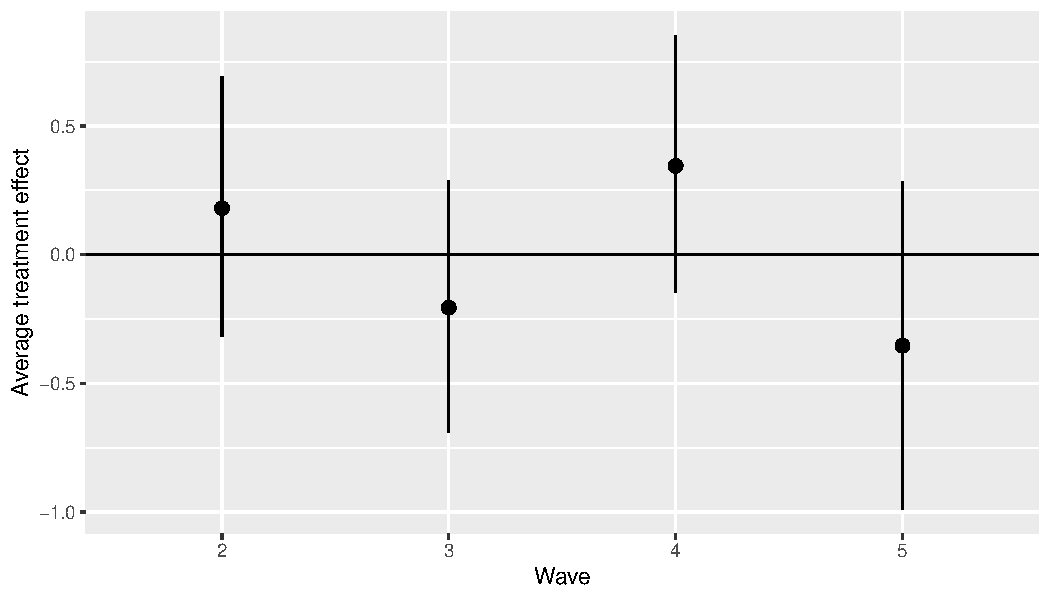
\includegraphics[width=0.5\linewidth,]{../figures/lsat_teff} 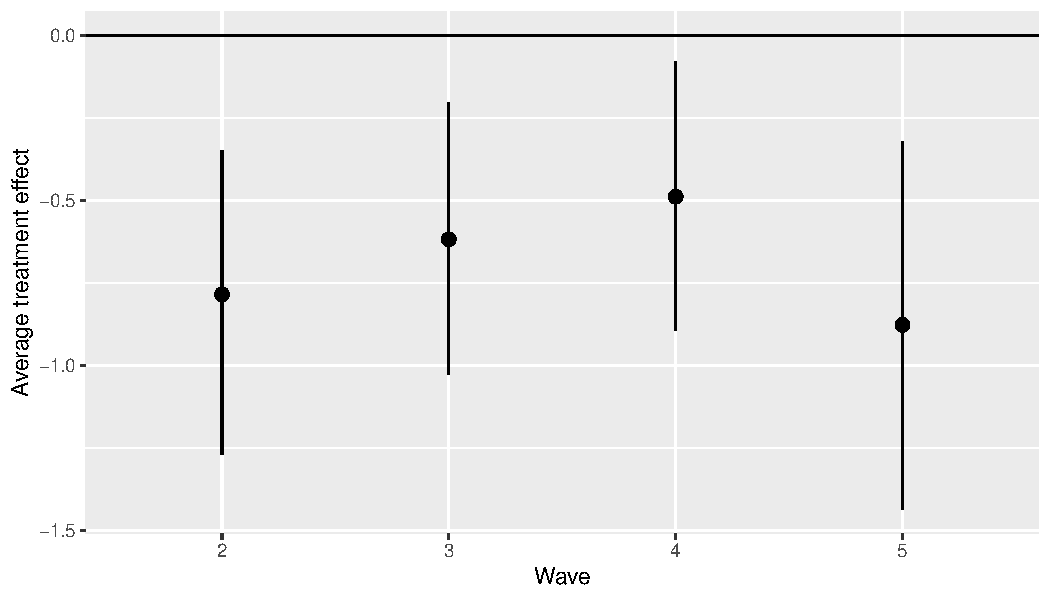
\includegraphics[width=0.5\linewidth,]{../figures/sat_friends_teff} 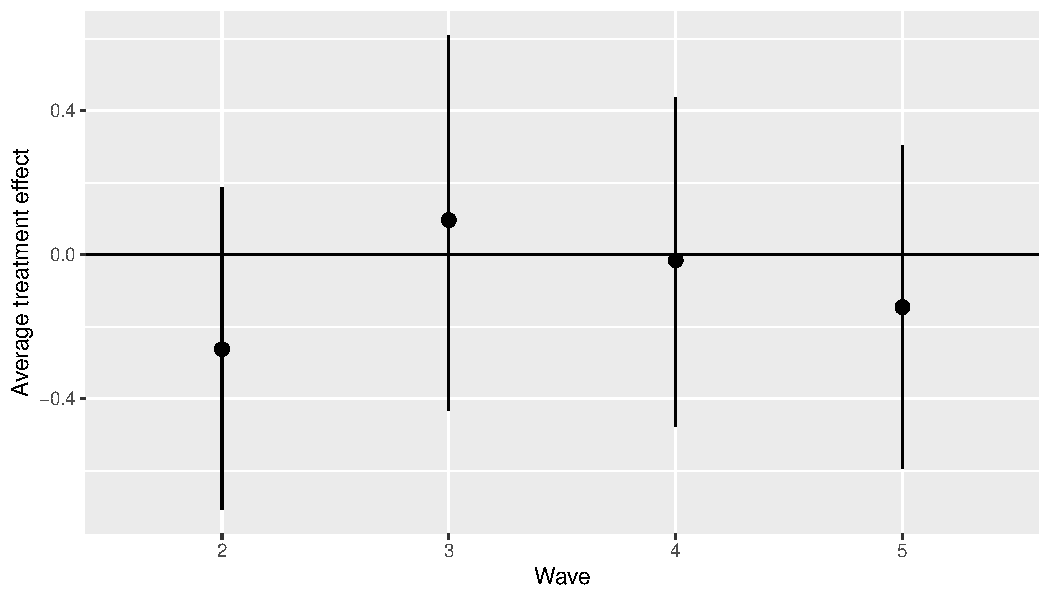
\includegraphics[width=0.5\linewidth,]{../figures/sat_class_teff} 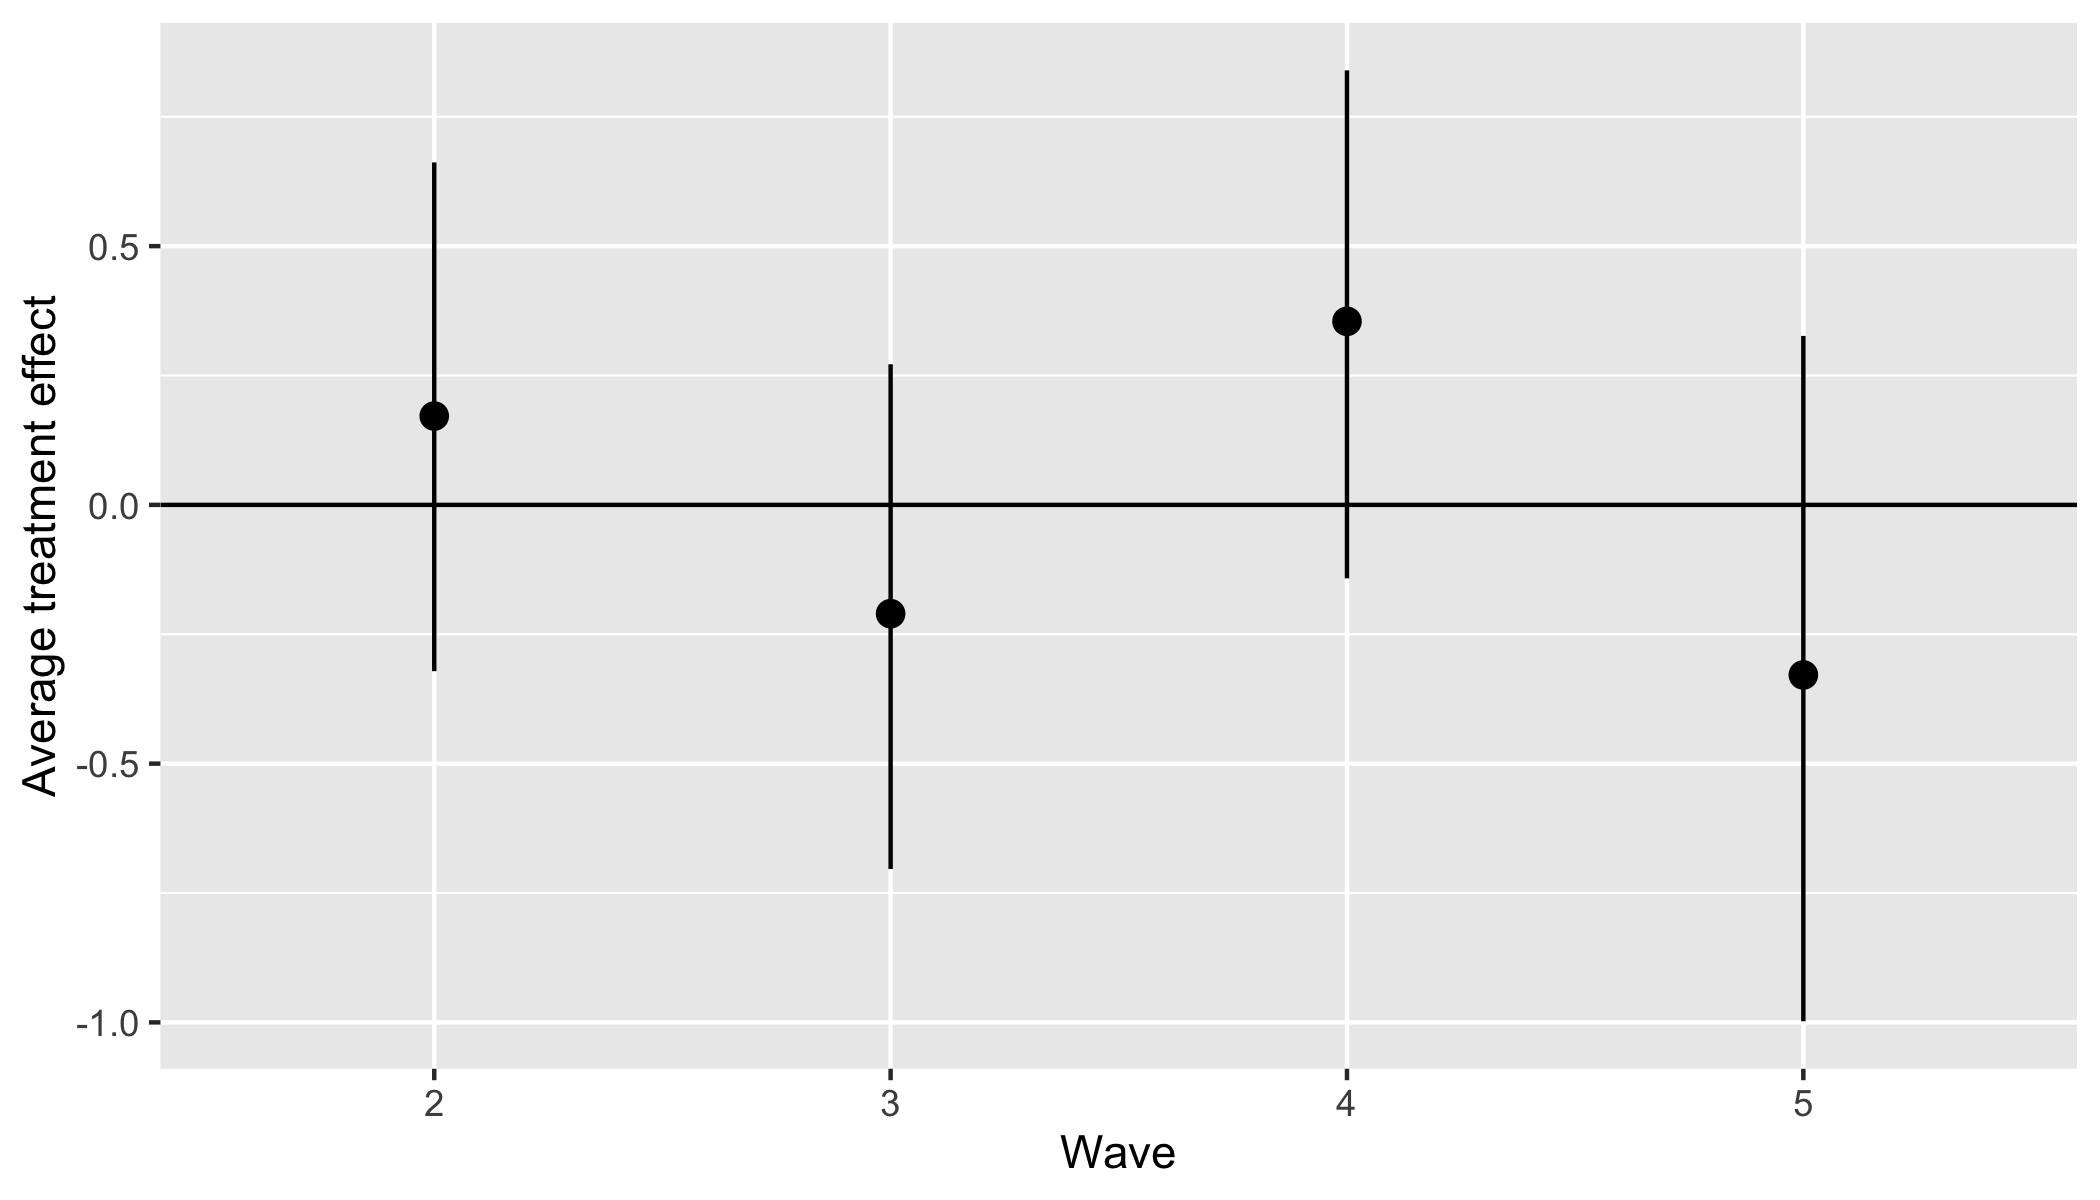
\includegraphics[width=0.5\linewidth,]{../figures/sat_school_teff} \caption{Treatment effects by area of satisfaction for average school}\label{fig:sat-teff}
\end{figure}

\hypertarget{across-schools}{%
\subsubsection{Across schools}\label{across-schools}}

The pattern from Figure \ref{fig:lsat-teff} also appears in Figure \ref{fig:lsat-teff-across-schools}: There is a tendency of the treatment effects alternating from positive to negative from one wave to another. The magnitude of the effects however is extremely small and the 90\% credibility intervals always cross the zero line. Wave 5 paints a diffuse picture where school five seems to be completely off. The problem of school five being not very trustworthy was already mentioned when the descriptive statistics were introduced in Section \ref{sec:variables}.

\begin{figure}[H]

{\centering 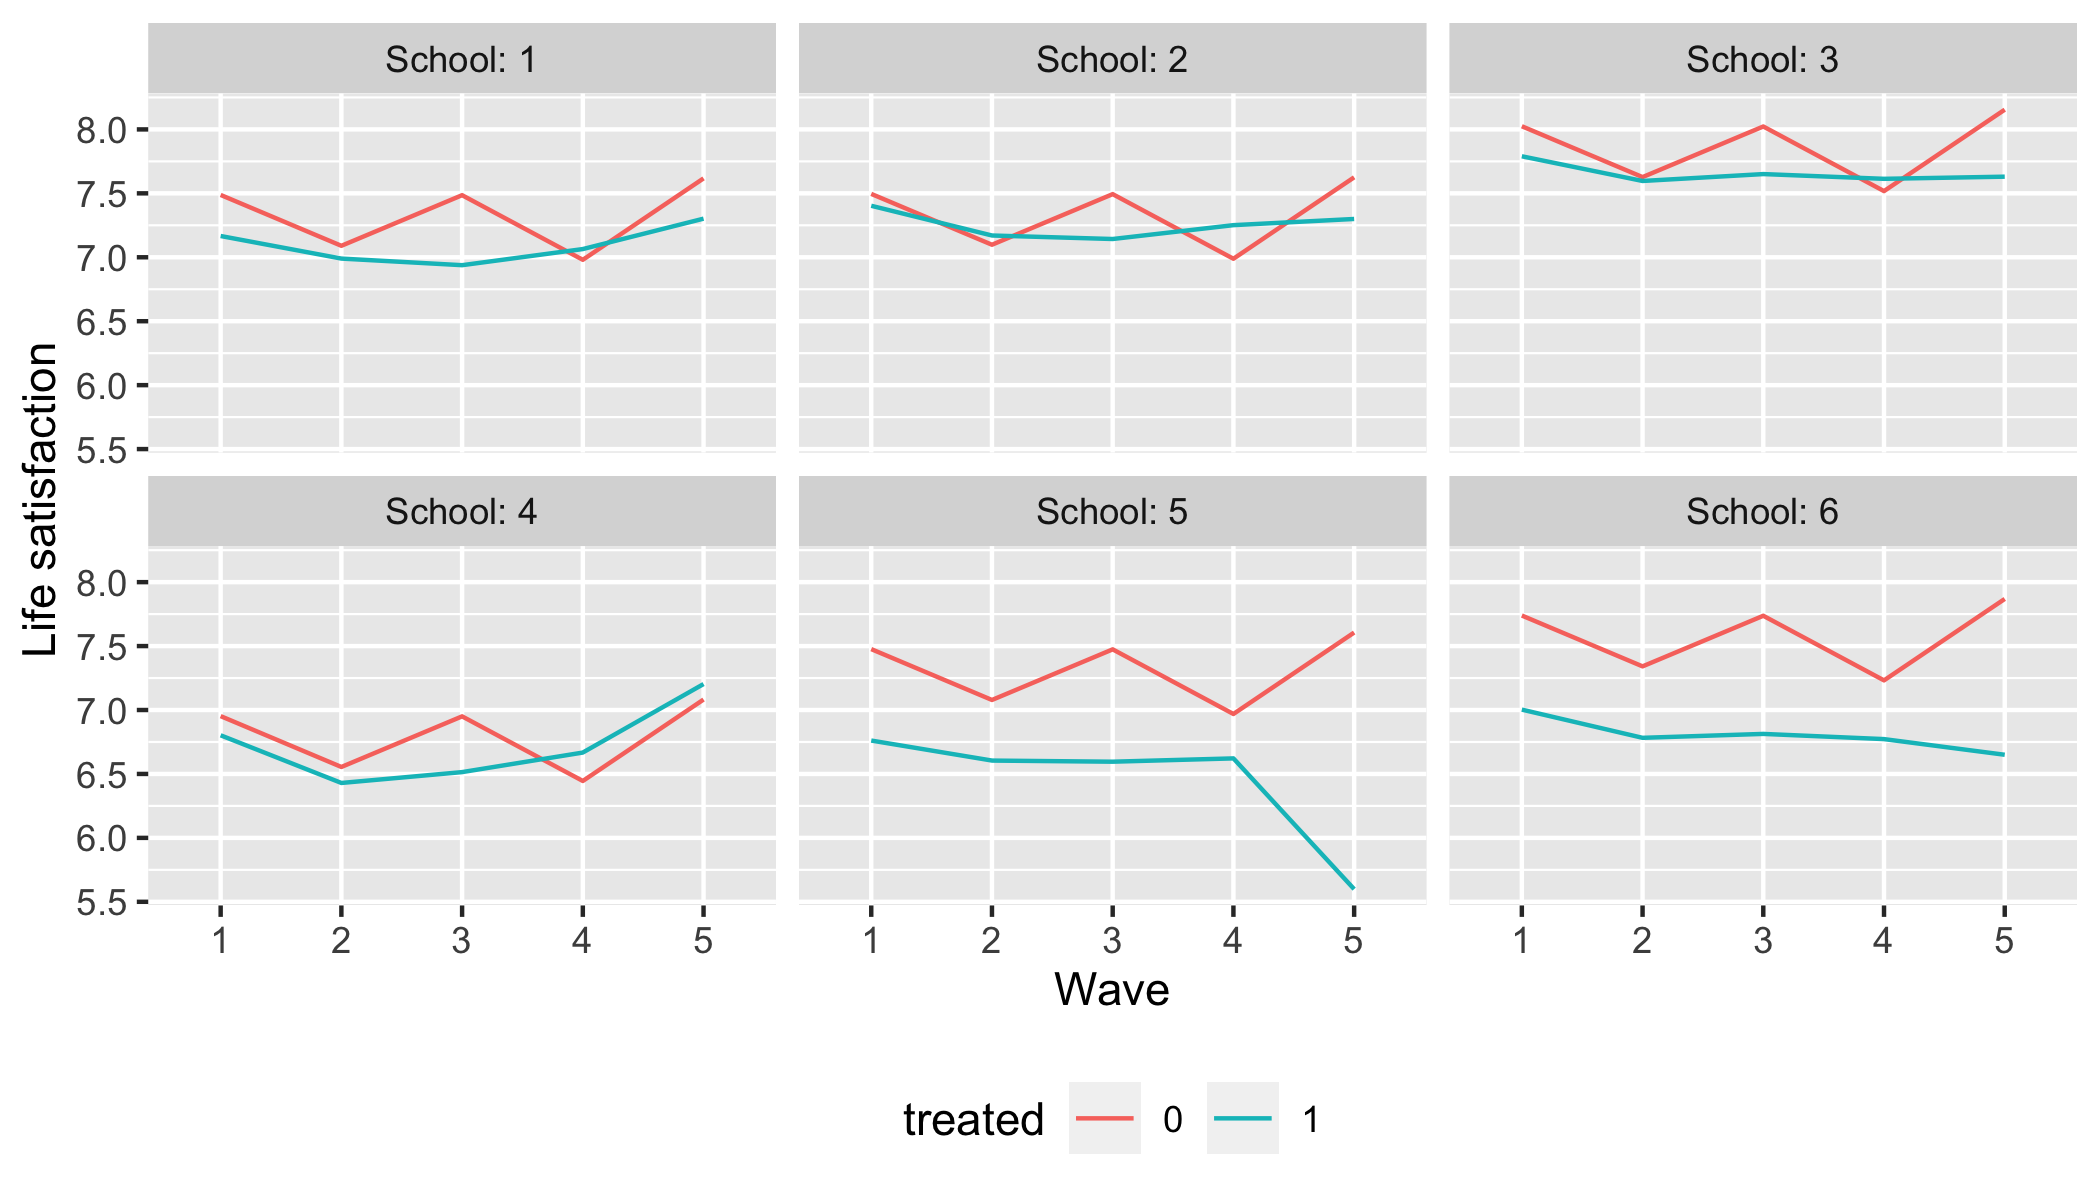
\includegraphics[width=0.8\linewidth,]{../figures/lsat_pred_across_schools} 

}

\caption{Predicted life satisfaction across schools}\label{fig:lsat-pred-across-schools}
\end{figure}

\begin{figure}[H]

{\centering 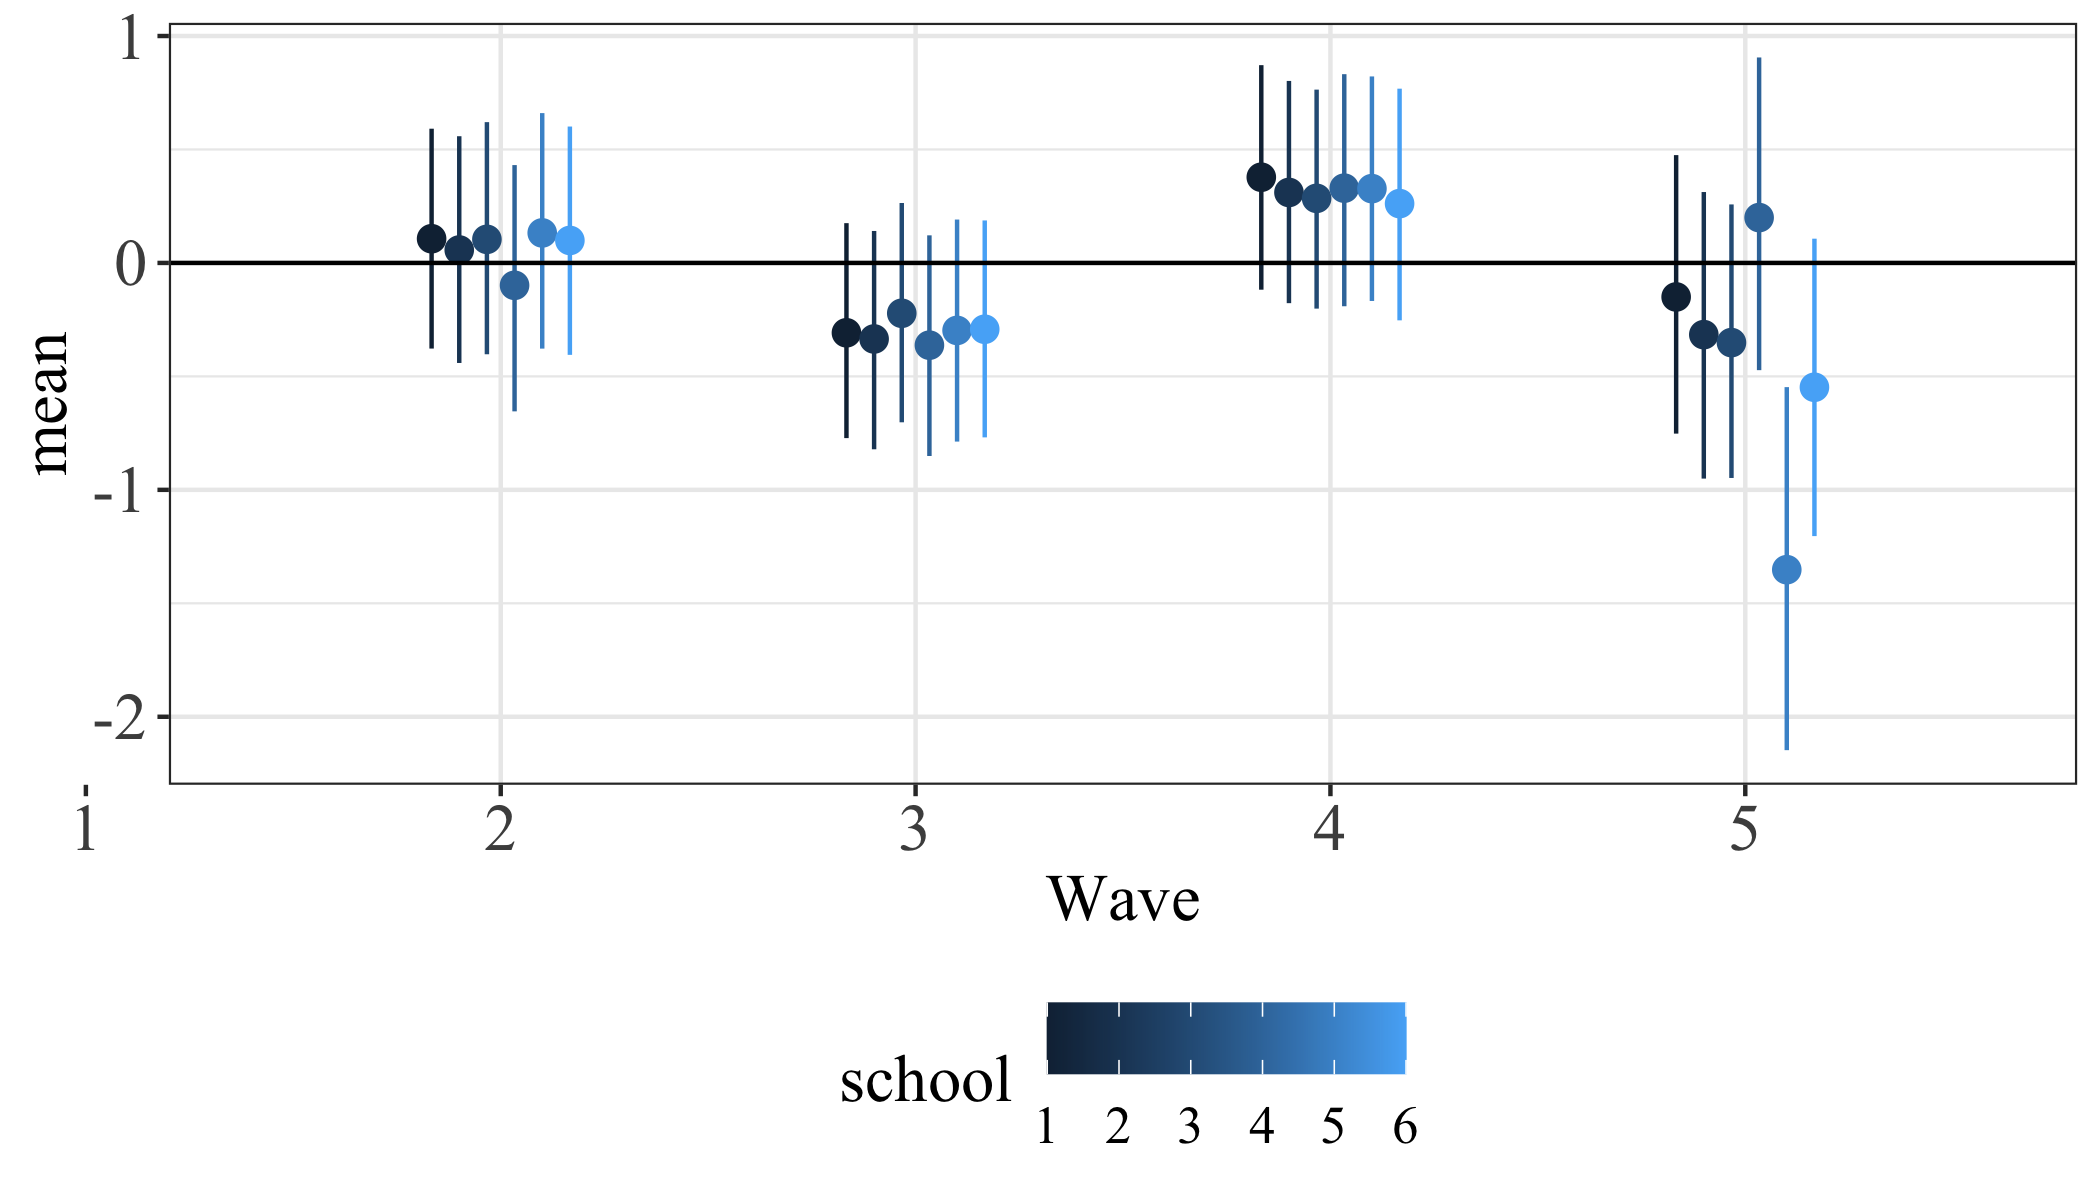
\includegraphics[width=0.8\linewidth,]{../figures/lsat_teff_across_schools} 

}

\caption{Treatment effects across schools}\label{fig:lsat-teff-across-schools}
\end{figure}

\hypertarget{satisfaction-with-friends}{%
\subsection{Satisfaction with friends}\label{satisfaction-with-friends}}

\label{sec:results-friends}
The area of satisfaction with friends is the only one, where clearly a negative effect was observed. In both of the groups, the students tend to become less satisfied with their friends. The control group becomes a little more satisfied in wave 2 compared to the previous wave but then drops by the same amount. It then stays on the same level of about 8.75. The treatment group drops consistently, being less satisfied with friends from period to period. The treatment group starts with a mean satisfaction at more than 9, which is the highest values observed in all of the areas, and reaches a level of even less than 8.25 in wave 5. The treatment effects are all below zero including the 90\% credibility intervals. Again, it is school 5 where the treatment group shows the most rapid drop in satisfaction with friends from 9 in wave 1 to 7.5 in wave 5. The other schools show also a decrease in their satisfaction levels but school 1 and school 3 show a tendency for increasing satisfaction to the end of the project.

\hypertarget{satisfaction-with-the-class}{%
\subsection{Satisfaction with the class}\label{satisfaction-with-the-class}}

\label{sec:results-class}
Averaging over all schools shows similar developments of the satisfaction with the class in the treatment and the control group. Both of them drop sharply in the first two periods and then remain on a level of around seven with the treatment group generally showing slightly lower satisfaction levels than the control group. Basically, the treatment effects are not significantly different from zero.
When looking at each school separately, there is no feature worth mentioning with the exception that in school 1 and 2, it is the students in the treatment class that are happier than the one in the control group on average.

\hypertarget{satisfaction-with-school}{%
\subsection{Satisfaction with school}\label{satisfaction-with-school}}

\label{sec:results-school}
The level of satisfaction with school is quite volatile throughout the time of the project. There is a pattern observable in the control group which shows that students are more satisfied with school at the beginning and at the end of a school year and less satisfied in between. The students in the treatment group generally show a level of satisfaction of more than eight and around 7/7.25 in all the other periods. The drop from wave 1 to wave 2 can be seen in each of the observed schools. But while in the other schools, it goes up again after that initial drop and eventually levels, school 5 is the only school where it continues to drop for the treatment group and goes even down to below 6 which can be categorized as dissatisfied.

\clearpage

\hypertarget{conclusion}{%
\section{Conclusion}\label{conclusion}}

\label{ch:conclusion}

\begin{figure}[H]

{\centering 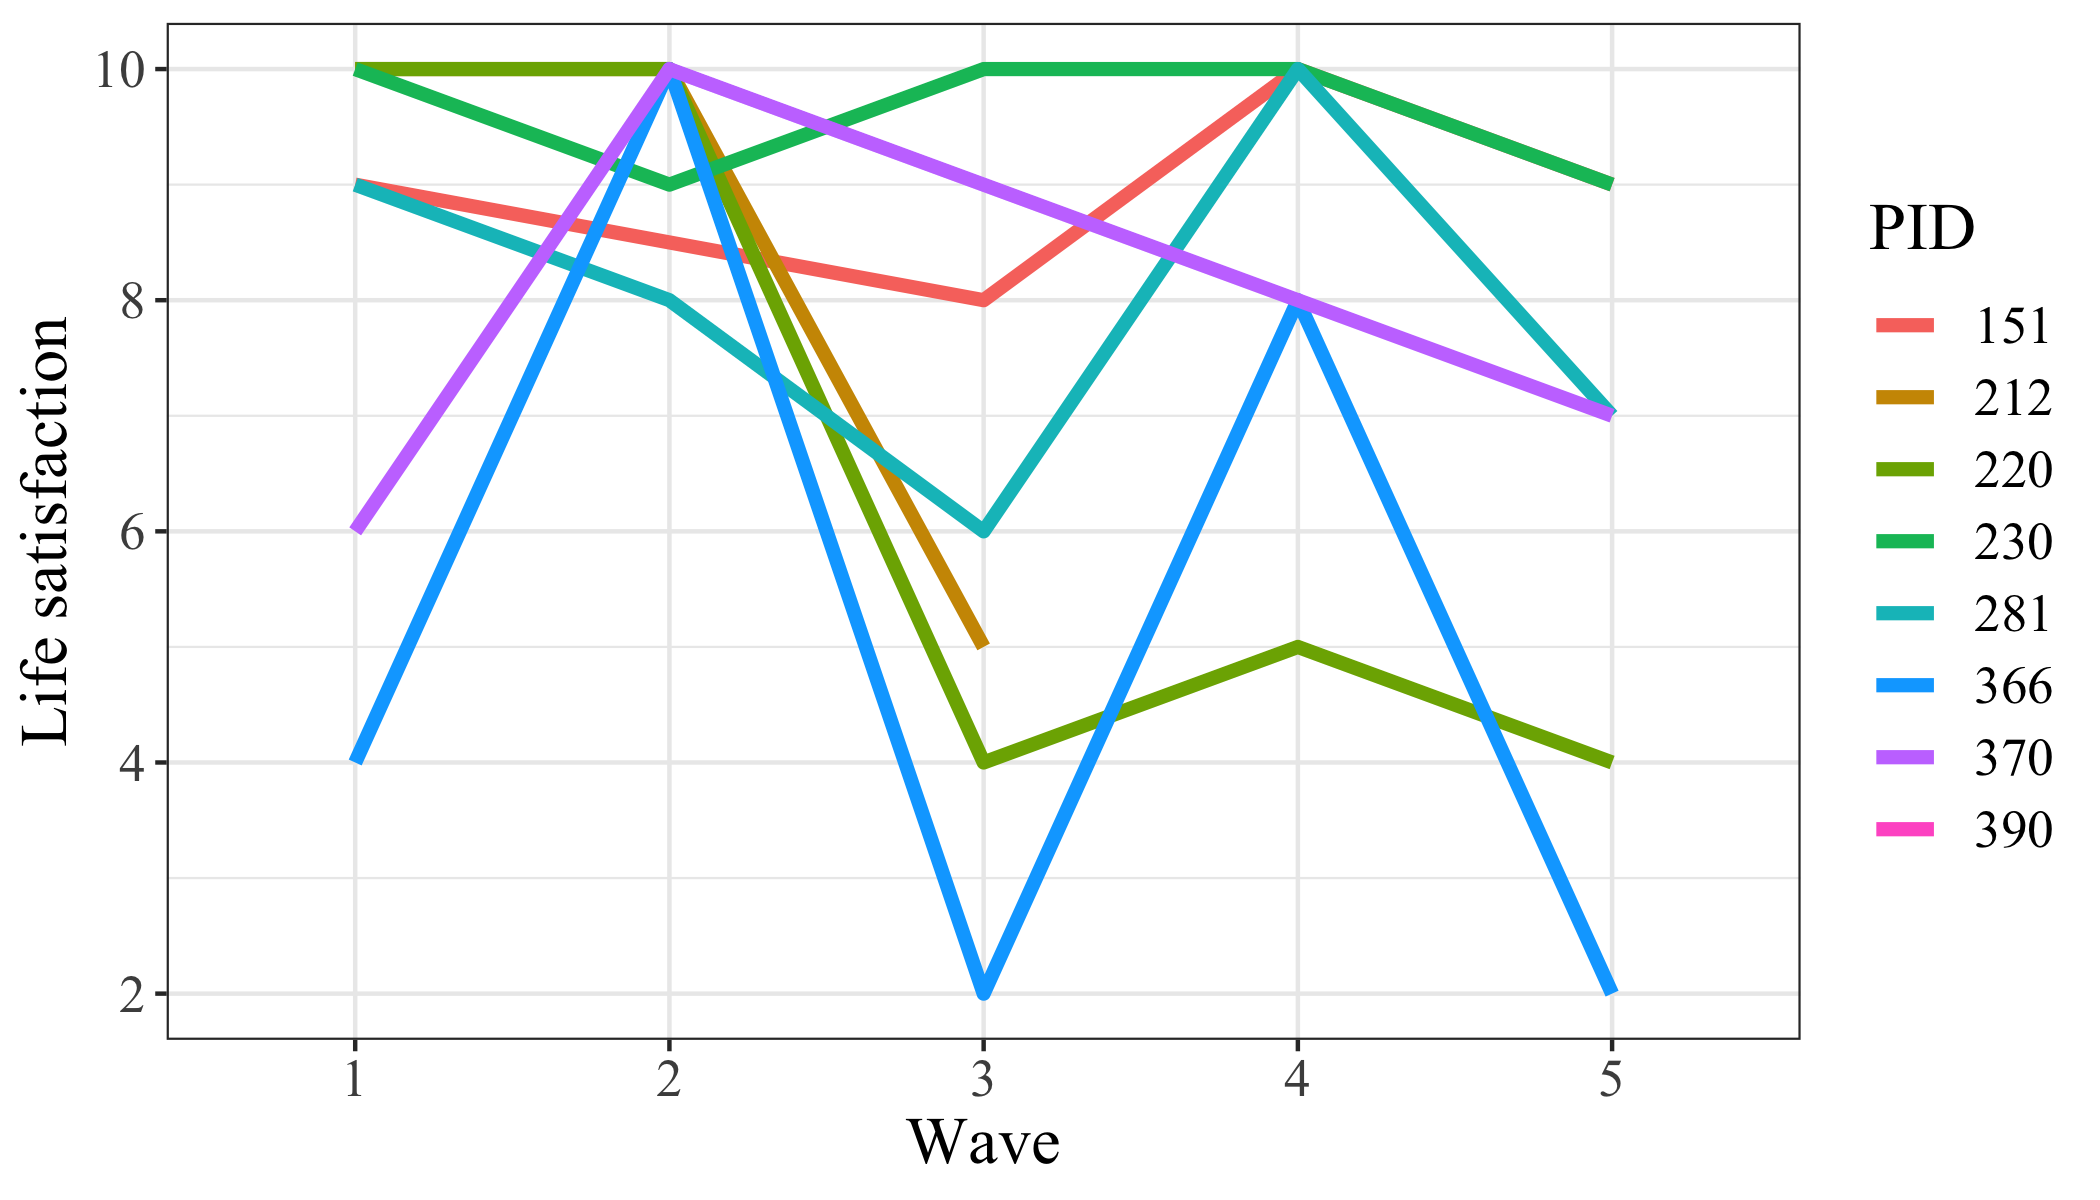
\includegraphics[width=0.8\linewidth,]{../figures/random_lsat} 

}

\caption{Excerpt from questionnaire}\label{fig:random-pid}
\end{figure}

\clearpage

\hypertarget{references}{%
\section*{References}\label{references}}
\addcontentsline{toc}{section}{References}

\singlespacing

\setlength{\parindent}{-0.5in}
\setlength{\leftskip}{0.5in}
\setlength{\parskip}{8pt}

\noindent

\hypertarget{refs}{}
\leavevmode\hypertarget{ref-Adelman1989}{}%
Adelman, H. S., Taylor, L., \& Nelson, P. (1989). Minors dissatisfaction with their life circumstances. \emph{Child Psychiatry \& Human Development}, \emph{20}(2), 135--147. \url{https://doi.org/10.1007/bf00711660}

\leavevmode\hypertarget{ref-AndrewGelman2013}{}%
Andrew Gelman, J. H. (2013). \emph{Data analysis using regression and multilevel/hierarchical models}. Retrieved from \url{https://www.ebook.de/de/product/6522123/andrew_gelman_jennifer_hill_data_analysis_using_regression_and_multilevel_hierarchical_models.html}

\leavevmode\hypertarget{ref-BundesverbandMusikunterricht}{}%
Bundesverband Musikunterricht (BMU). (2016). \emph{Grundsdatzpapier}. Retrieved from \url{https://www.bmu-musik.de/ueber-uns/positionen/agenda-2030-bmu-positionen-9-2016.html}

\leavevmode\hypertarget{ref-Buerkner2017}{}%
Bürkner, P.-C. (2017). Brms: An r package for bayesian multilevel models using stan. \emph{Journal of Statistical Software}, \emph{80}(1). \url{https://doi.org/10.18637/jss.v080.i01}

\leavevmode\hypertarget{ref-Casas2015}{}%
Casas, F., \& Rees, G. (2015). Measures of children's subjective well-being: Analysis of the potential for cross-national comparisons. \emph{Child Indicators Research}, \emph{8}(1), 49--69. \url{https://doi.org/10.1007/s12187-014-9293-z}

\leavevmode\hypertarget{ref-Casas2011}{}%
Casas, F., Sarriera, J. C., Alfaro, J., González, M., Malo, S., Bertran, I., \ldots{} Valdenegro, B. (2011). Testing the personal wellbeing index on 1216~year-old adolescents in 3 different countries with 2 new items. \emph{Social Indicators Research}, \emph{105}(3), 461--482. \url{https://doi.org/10.1007/s11205-011-9781-1}

\leavevmode\hypertarget{ref-Johnston2002}{}%
Chambers, C. T., \& Johnston, C. (2002). Developmental differences in childrens use of rating scales. \emph{Journal of Pediatric Psychology}, \emph{27}(1), 27--36. \url{https://doi.org/10.1093/jpepsy/27.1.27}

\leavevmode\hypertarget{ref-Cheung2014}{}%
Cheung, F., \& Lucas, R. E. (2014). Assessing the validity of single-item life satisfaction measures: Results from three large samples. \emph{Quality of Life Research}, \emph{23}(10), 2809--2818. \url{https://doi.org/10.1007/s11136-014-0726-4}

\leavevmode\hypertarget{ref-CostaGiomi2004}{}%
Costa-Giomi, E. (2004). Effects of three years of piano instruction on children's academic achievement, school performance and self-esteem. \emph{Psychology of Music}, \emph{32}(2), 139--152. \url{https://doi.org/10.1177/0305735604041491}

\leavevmode\hypertarget{ref-Cummins1997}{}%
Cummins, R. A. (1997). \emph{Manual for the comprehensive quality of life scale -- student (grades 7-12): ComQol-s5} (5th ed.). Malbourne: Deakin University, School of Psychology.

\leavevmode\hypertarget{ref-Cummins2005}{}%
Cummins, R. A., \& Lau, A. L. D. (2005). \emph{Personal wellbeing index - school children (PWI-SC)} (3rd ed.). Australian Centre on Quality of Life, School of Psychology, Deakin University, Australia.

\leavevmode\hypertarget{ref-Diener2009}{}%
Diener, E. (2009). \emph{Culture and well-being} (T. Moum, M. A. G. Sprangers, J. Vogel, R. V. C. Michalos, E. Diener, \& W. G. and, Eds.). \url{https://doi.org/10.1007/978-90-481-2352-0}

\leavevmode\hypertarget{ref-Diener1985}{}%
Diener, E., Emmons, R. A., Larsen, R. J., \& Griffin, S. (1985). The satisfaction with life scale. \emph{Journal of Personality Assessment}, \emph{49}(1), 71--75. \url{https://doi.org/10.1207/s15327752jpa4901_13}

\leavevmode\hypertarget{ref-iCarbonell2004}{}%
Ferrer-i-Carbonell, A., \& Frijters, P. (2004). How important is methodology for the estimates of the determinants of happiness? \emph{The Economic Journal}, \emph{114}(497), 641--659. \url{https://doi.org/10.1111/j.1468-0297.2004.00235.x}

\leavevmode\hypertarget{ref-Gebert2018}{}%
Gebert, S. (2018). \emph{Musische erziehung ist keine privatangelegenheit}. Retrieved from \url{https://www.deutschlandfunk.de/musikunterricht-an-schulen-musische-erziehung-ist-keine.680.de.html?dram:article_id=419333}

\leavevmode\hypertarget{ref-Gilman2000}{}%
Gilman, R., \& Huebner, E. S. (2000). Review of life satisfaction measures for adolescents. \emph{Behaviour Change}, \emph{17}(3), 178--195. \url{https://doi.org/10.1375/bech.17.3.178}

\leavevmode\hypertarget{ref-Gilman2006}{}%
Gilman, R., \& Huebner, E. S. (2006). Characteristics of adolescents who report very high life satisfaction. \emph{Journal of Youth and Adolescence}, \emph{35}(3), 293--301. \url{https://doi.org/10.1007/s10964-006-9036-7}

\leavevmode\hypertarget{ref-Gluskie2012}{}%
Gluskie, A. L. (2012). \emph{Subjective wellbeing in children} (PhD thesis). Deakin University.

\leavevmode\hypertarget{ref-GonzalezCarrasco2016}{}%
González-Carrasco, M., Casas, F., Malo, S., Viñas, F., \& Dinisman, T. (2016). Changes with age in subjective well-being through the adolescent years: Differences by gender. \emph{Journal of Happiness Studies}, \emph{18}(1), 63--88. \url{https://doi.org/10.1007/s10902-016-9717-1}

\leavevmode\hypertarget{ref-Guhn2019}{}%
Guhn, M., Emerson, S. D., \& Gouzouasis, P. (2019). A population-level analyses of associations between school music participation and academic achievement. \emph{Journal of Educational Psychology}, \emph{112}(2), 308--328. \url{https://doi.org/http://dx.doi.org/10.1037/edu0000376}

\leavevmode\hypertarget{ref-Gullone1999}{}%
Gullone, E., \& Cummins, R. (1999). The comprehensive quality of life scale: A psychometric evaluation with an adolescent sample. \emph{Behaviour Change}, \emph{16}, 127--139.

\leavevmode\hypertarget{ref-Hille2014}{}%
Hille, J., Adrian; Schupp. (2014). How learning a musical instrument affects the development of skills. \emph{Economics of Education Review}, \emph{44}, 56--82. \url{https://doi.org/http://dx.doi.org/10.1016/j.econedurev.2014.10.007}

\leavevmode\hypertarget{ref-Huebner1991}{}%
Huebner, E. S. (1991a). Correlates of life satisfaction in children. \emph{School Psychology Quarterly}, \emph{6}(2), 103--111. \url{https://doi.org/https://doi.org/10.1037/h0088805}

\leavevmode\hypertarget{ref-Huebner1991a}{}%
Huebner, E. S. (1991b). Initial development of the students life satisfaction scale. \emph{School Psychology International}, \emph{12}(3), 231--240. \url{https://doi.org/10.1177/0143034391123010}

\leavevmode\hypertarget{ref-Huebner1994}{}%
Huebner, E. S. (1994). Preliminary development and validation of a multidimensional life satisfaction scale for children. \emph{Psychological Assessment}, \emph{6}(2), 149--158. \url{https://doi.org/10.1037/1040-3590.6.2.149}

\leavevmode\hypertarget{ref-Kim2003}{}%
Kim, K. J., Conger, R. D., Elder, G. H., \& Lorenz, F. O. (2003). Reciprocal influences between stressful life events and adolescent internalizing and externalizing problems. \emph{Child Development}, \emph{74}(1), 127--143. \url{https://doi.org/10.1111/1467-8624.00525}

\leavevmode\hypertarget{ref-Marsh1986}{}%
Marsh, H. W. (1986). Negative item bias in ratings scales for preadolescent children: A cognitive-developmental phenomenon. \emph{Developmental Psychology}, \emph{22}(1), 37--49. \url{https://doi.org/10.1037/0012-1649.22.1.37}

\leavevmode\hypertarget{ref-Mcelreath2020}{}%
Mcelreath, R. (2020). \emph{Statistical rethinking}. Retrieved from \url{https://www.ebook.de/de/product/38708673/richard_mcelreath_statistical_rethinking.html}

\leavevmode\hypertarget{ref-Mehr2013}{}%
Mehr, S. A., Schachner, A., Katz, R. C., \& Spelke, E. S. (2013). Two randomized trials provide no consistent evidence for nonmusical cognitive benefits of brief preschool music enrichment. \emph{PLoS ONE}, \emph{8}(12), e82007. \url{https://doi.org/10.1371/journal.pone.0082007}

\leavevmode\hypertarget{ref-Mellor2008}{}%
Mellor, D., Stokes, M., Firth, L., Hayashi, Y., \& Cummins, R. (2008). Need for belonging, relationship satisfaction, loneliness, and life satisfaction. \emph{Personality and Individual Differences}, \emph{45}(3), 213--218. \url{https://doi.org/10.1016/j.paid.2008.03.020}

\leavevmode\hypertarget{ref-Moeller2017}{}%
Möller, T. (2017). \emph{Ausverkauf musikalischer Bildung?} Retrieved from \url{https://www.deutschlandfunk.de/musikunterricht-in-der-schule-ausverkauf-musikalischer.1992.de.html?dram:article_id=382783}

\leavevmode\hypertarget{ref-Osborne2015}{}%
Osborne, M. S., McPherson, G. E., Faulkner, R., Davidson, J. W., \& Barrett, M. S. (2015). Exploring the academic and psychosocial impact of el sistema-inspired music programs within two low socio-economic schools. \emph{Music Education Research}, \emph{18}(2), 156--175. \url{https://doi.org/10.1080/14613808.2015.1056130}

\leavevmode\hypertarget{ref-Piaget1955}{}%
Piaget, J. (1955). \emph{The construction of reality in the child}. London: Routledge; Keagan Paul.

\leavevmode\hypertarget{ref-Piaget1969}{}%
Piaget, J. (1969). \emph{The child's concept of time}. London: Routledge; Keagan Paul.

\leavevmode\hypertarget{ref-Portowitz2009}{}%
Portowitz, A., Lichtenstein, O., Egorova, L., \& Brand, E. (2009). Underlying mechanisms linking music education and cognitive modifiability. \emph{Research Studies in Music Education}, \emph{31}(2), 107--128. \url{https://doi.org/10.1177/1321103x09344378}

\leavevmode\hypertarget{ref-Proctor2009a}{}%
Proctor, C., Linley, P. A., \& Maltby, J. (2009). Very happy youths: Benefits of very high life satisfaction among adolescents. \emph{Social Indicators Research}, \emph{98}(3), 519--532. \url{https://doi.org/10.1007/s11205-009-9562-2}

\leavevmode\hypertarget{ref-Rubin1981}{}%
Rubin, D. B. (1981). Estimation in parallel randomized experiments. \emph{Journal of Educational Statistics}, \emph{6}(4), 377--401. \url{https://doi.org/10.3102/10769986006004377}

\leavevmode\hypertarget{ref-Sala2016}{}%
Sala, G., \& Gobet, F. (2016). When the musics over. Does music skill transfer to childrens and young adolescents cognitive and academic skills? A meta-analysis. \emph{Educational Research Review}, \emph{20}, 55--67. \url{https://doi.org/10.1016/j.edurev.2016.11.005}

\leavevmode\hypertarget{ref-Schellenberg2004}{}%
Schellenberg, E. G. (2004). Music lessons enhance IQ. \emph{Psychological Science}, \emph{15}(8), 511--514. \url{https://doi.org/https://doi.org/10.1111/j.0956-7976.2004.00711.x}

\leavevmode\hypertarget{ref-Schellenberg2011a}{}%
Schellenberg, E. G. (2011). Music lessons, emotional intelligence, and IQ. \emph{Music Perception: An Interdisciplinary Journal}, \emph{29}(2), 185--194. \url{https://doi.org/10.1525/mp.2011.29.2.185}

\leavevmode\hypertarget{ref-Schellenberg2013}{}%
Schellenberg, E. G., \& Weiss, M. W. (2013). Music and cognitive abilities. In \emph{The psychology of music} (pp. 499--550). \url{https://doi.org/10.1016/b978-0-12-381460-9.00012-2}

\leavevmode\hypertarget{ref-Southgate2009}{}%
Southgate, D. E., \& Roscigno, V. J. (2009). The impact of music on childhood and adolescent achievement. \emph{Social Science Quarterly}, \emph{90}(1), 4--21. \url{https://doi.org/10.1111/j.1540-6237.2009.00598.x}

\leavevmode\hypertarget{ref-Stoverock}{}%
Stoverock, K. (n.d.). \emph{Ein jahrzehntelanges versagen der bildungspolitik}. Retrieved from \url{https://themen.miz.org/fokus-musikunterricht/interview-hoeppner}

\leavevmode\hypertarget{ref-Suldo2004}{}%
Suldo, S. M., \& Huebner, E. S. (2004). Does life satisfaction moderate the effects of stressful life events on psychopathological behavior during adolescence? \emph{School Psychology Quarterly}, \emph{19}(2), 93--105. \url{https://doi.org/10.1521/scpq.19.2.93.33313}

\leavevmode\hypertarget{ref-Tomyn2011a}{}%
Tomyn, A. J., \& Cummins, R. A. (2011). The subjective wellbeing of high-school students: Validating the personal wellbeing indexSchool children. \emph{Social Indicators Research}, \emph{101}(3), 405--418. \url{https://doi.org/10.1007/s11205-010-9668-6}

\leavevmode\hypertarget{ref-Tomyn2016}{}%
Tomyn, A. J., Fuller-Tyszkiewicz, M. D., Cummins, R. A., \& Norrish, J. M. (2016). The validity of subjective wellbeing measurement for children: Evidence using the personal wellbeing indexSchool children. \emph{Journal of Happiness Studies}, \emph{18}(6), 1859--1875. \url{https://doi.org/10.1007/s10902-016-9804-3}

\leavevmode\hypertarget{ref-Tomyn2019}{}%
Tomyn, A. J., Stokes, M. A., Cummins, R. A., \& Dias, P. C. (2019). A rasch analysis of the personal well-being index in school children. \emph{Evaluation \& the Health Professions}, \emph{43}(2), 110--119. \url{https://doi.org/10.1177/0163278718819219}

\leavevmode\hypertarget{ref-Uy2012}{}%
Uy, M. (2012). Venezuela's national music education program el sistema: Its interactions with society and its participants' engagement in praxis. \emph{Music \& Arts in Action}, \emph{4}(1), 5--21. Retrieved from \url{http://musicandartsinaction.net/index.php/maia/article/view/elsistema}

\leavevmode\hypertarget{ref-Valois2004}{}%
Valois, R. F., Zullig, K. J., Huebner, E. S., \& Drane, J. W. (2004). Life satisfaction and suicide among high school adolescents. \emph{Social Indicators Research}, \emph{66}(1/2), 81--105. \url{https://doi.org/10.1023/b:soci.0000007499.19430.2f}

\leavevmode\hypertarget{ref-Wetter2008}{}%
Wetter, O. E., Koerner, F., \& Schwaninger, A. (2008). Does musical training improve school performance? \emph{Instructional Science}, \emph{37}(4), 365--374. \url{https://doi.org/10.1007/s11251-008-9052-y}

\leavevmode\hypertarget{ref-Yang2015}{}%
Yang, P. (2015). The impact of msic on educational attainment. \emph{Journal of Cultural Economics}, \emph{39}(4), 369--396. \url{https://doi.org/10.1007/s10824-015-9240-y}

\leavevmode\hypertarget{ref-Zullig2001}{}%
Zullig, K. J., Valois, R. F., Huebner, E. S., Oeltmann, J. E., \& Drane, J. W. (2001). Relationship between perceived life satisfaction and adolescents' substance abuse. \emph{Journal of Adolescent Health}, \emph{29}(4), 279--288. \url{https://doi.org/10.1016/s1054-139x(01)00269-5}

\clearpage

\hypertarget{appendix-appendix}{%
\appendix}


\hypertarget{appendix-a}{%
\section{Appendix A}\label{appendix-a}}

\begin{figure}[H]
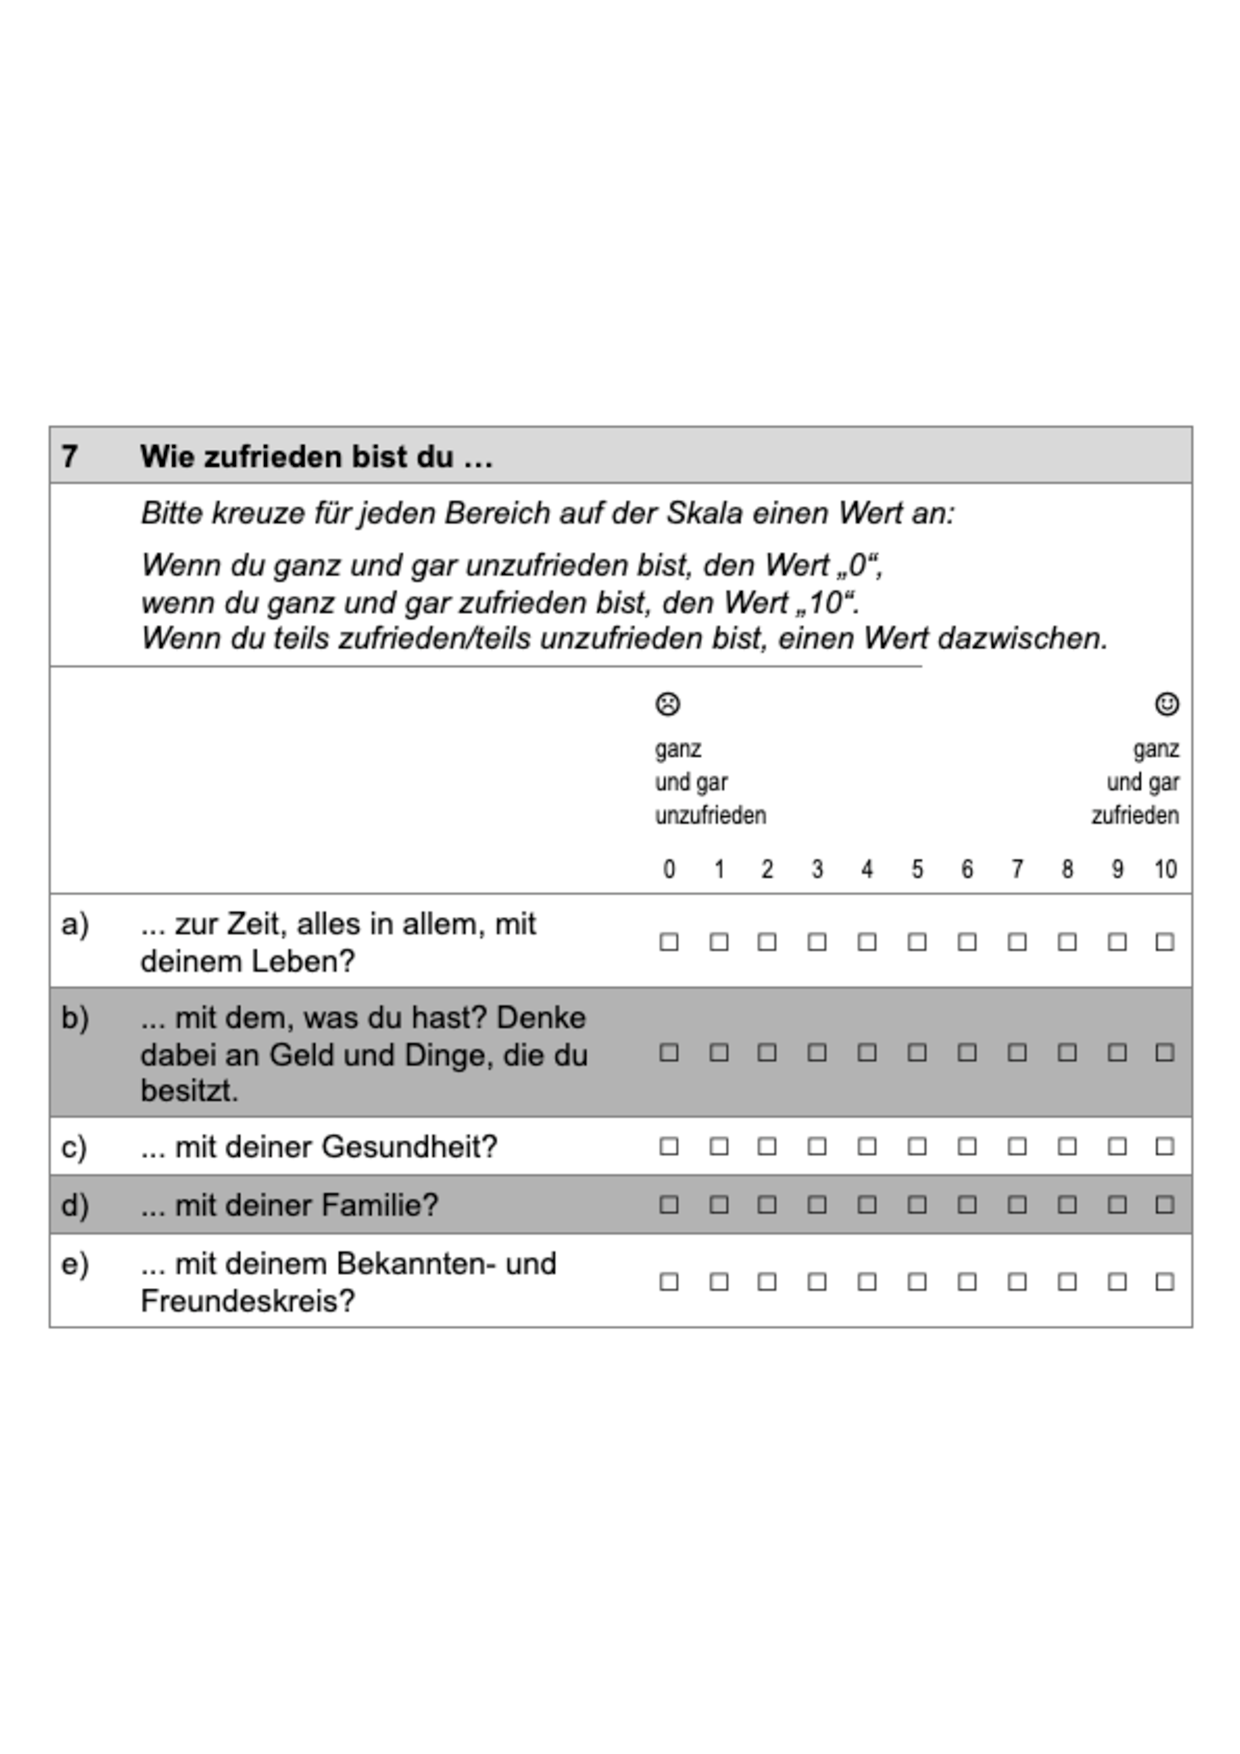
\includegraphics[width=1\linewidth,]{../figures/Wie zufrieden bist du....pdf} \caption{Excerpt from questionnaire}\label{fig:questionnaire}
\end{figure}
\begin{figure}[H]

{\centering 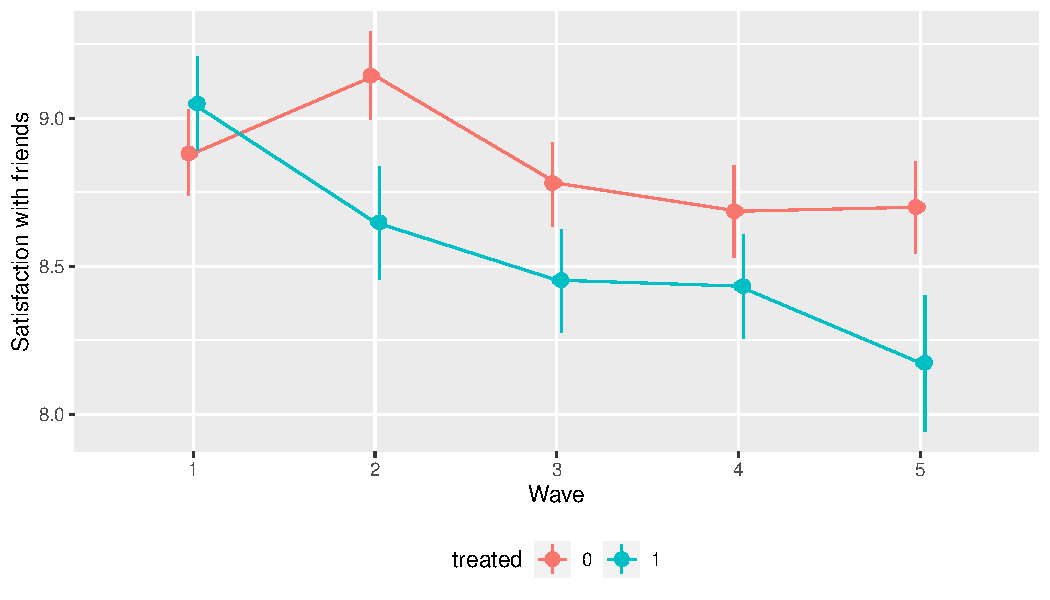
\includegraphics[width=0.65\linewidth,]{../figures/sat_friends_pred} 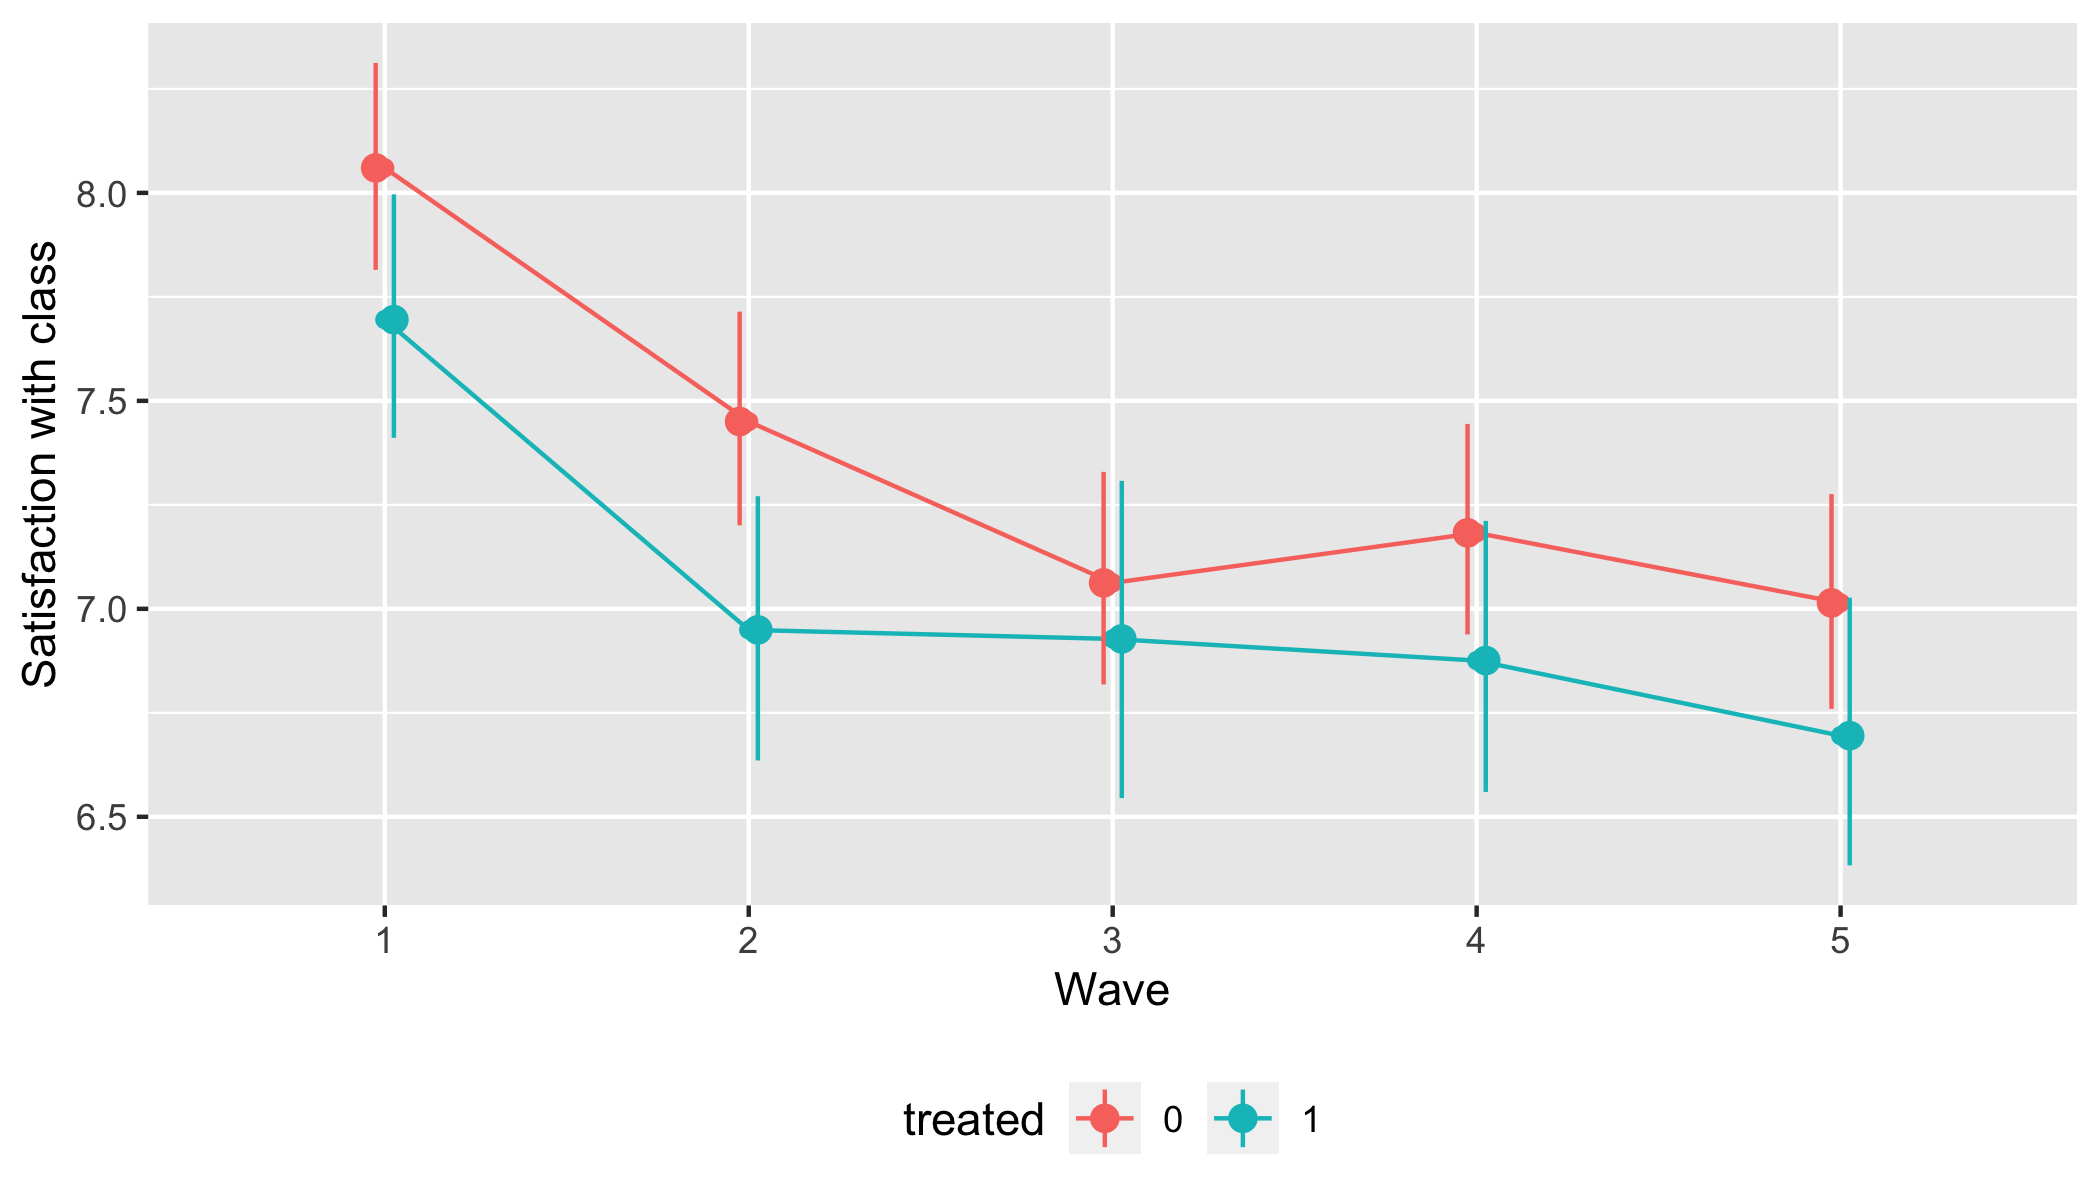
\includegraphics[width=0.65\linewidth,]{../figures/sat_class_pred} 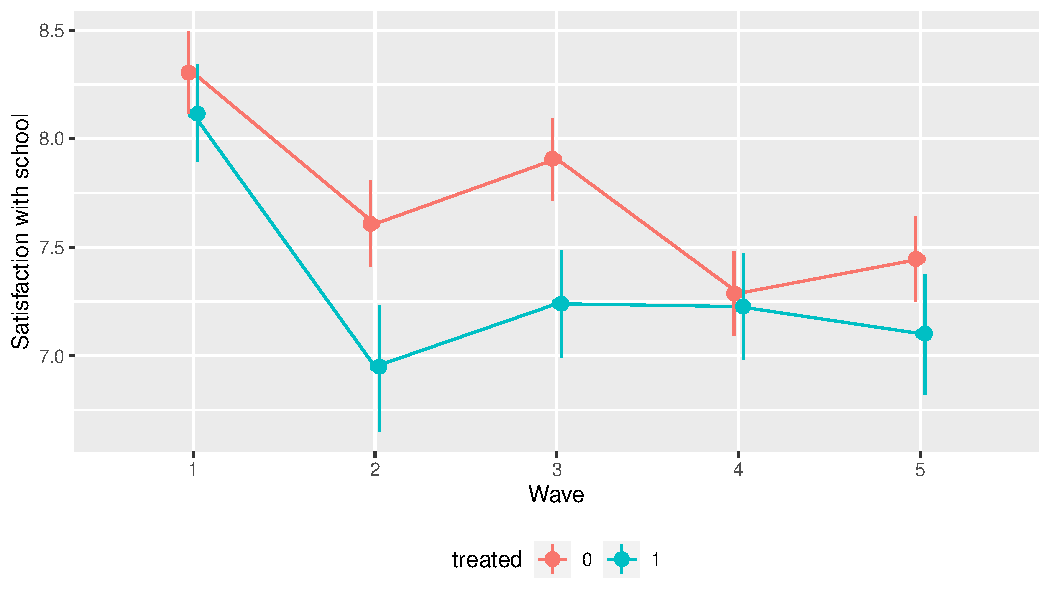
\includegraphics[width=0.65\linewidth,]{../figures/sat_school_pred} 

}

\caption{Predicted satisaction by area for average school}\label{fig:sat-pred}
\end{figure}

Example of nice appendix in Hille (2014)

\clearpage

\hypertarget{appendix-b}{%
\section{Appendix B}\label{appendix-b}}
\end{document}

